\section{Tổng quan về geometric deep learning}


\subsection{Mạng nơ-ron đồ thị và tiền thân hóa học của chúng}
Hóa học là một nhánh của khoa học tự nhiên nhằm nghiên cứu về thành phần, cấu trúc, tính chất, và sự thay đổi của vật chất. Các chủ đề chính trong hóa học là nguyên tố, hợp chất, nguyên tử, phân tử, và các phản ứng hóa học. Để nghiên cứu về các lĩnh vực này, các nhà hóa học cần phải nghiên cứu phản ứng hay công thức phân tử, ... Tuy nhiên, với sự phát triển của công nghệ thì giờ ta hoàn toàn có thể sử dụng tin học trong hóa học. Đầu tiên, ta sẽ bắt đầu từ tin học trong hóa học thời sơ khai.

Nó bắt đầu bằng nguồn gốc của hóa tin học, được đánh dấu bằng các ví dụ như "Chemisches Zentralblatt" (tạp chí tóm tắt hóa học đầu tiên), "Beilstein Handbuch" (một tập hợp toàn diện các hợp chất hữu cơ) và sự xuất hiện của Dịch vụ Tóm tắt Hóa học (CAS). Những nỗ lực sơ khai này đã nhấn mạnh nhu cầu sắp xếp và quản lý thông tin hóa học \cite{geometricdeep2022}.

Thẻ đục lỗ cho máy tính ban đầu biểu thị phương pháp sử dụng ban đầu máy tính trong hóa học, thiết lập nền tảng cho các phương pháp dựa trên dữ liệu hơn nữa\cite{geometricdeep2022}.

Tuy nhiên, việc biểu diễn và so sánh cấu trúc phân tử vẫn còn là một thách thức. Sơ đồ nêu bật những hạn chế của "mã hóa hóa học" ban đầu, vốn thường không nắm bắt được sự tương đồng về cấu trúc giữa các phân tử\cite{geometricdeep2022}. Một ví dụ được đưa ra với hai phân tử được biểu diễn bằng các ký hiệu tuyến tính khác nhau trong khi có chung cấu trúc.

Tiếp theo, báo cáo đưa ra mối liên thệ giữa lý thuyết đồ thị và hóa học. Năm 1878, James J. Sylvester đã ghi nhận mối quan hệ giữa hóa học và lý thuyết đồ thị\cite{geometricdeep2022}. Ông đã giới thiệu thuật ngữ "đồ thị" trong bối cảnh hóa học, nhận ra rằng cấu trúc phân tử có thể được biểu diễn hiệu quả bằng đồ thị. Ý tưởng có tầm nhìn xa này đã đặt nền móng cho các biểu diễn phân tử dựa trên đồ thị.

Dưới đây là một số nhà khoa học đã đóng góp để tạo ra mạng nơ-ron đồ thị đầu tiên:
\begin{itemize}
    \item Alessandro Sperduti (1994): Làm việc trên việc gán nhãn RAAM, một kiến trúc mạng nơ-ron cho dữ liệu có cấu trúc đồ thị\cite{geometricdeep2022}.
    
    \item Christoph Goller (1996): Khám phá lan truyền ngược thông qua cấu trúc, điều này rất quan trọng để huấn luyện GNN\cite{geometricdeep2022}.

    \item Kristian Kersting và các đồng nghiệp: Giới thiệu thuật ngữ "Mạng nơ-ron đồ thị" và phát triển các kiến trúc GNN hơn nữa\cite{geometricdeep2022}.

    \item Yujia Li (2015): Làm việc trên Gated GNN, giúp nâng cao việc biểu diễn đồ thị\cite{geometricdeep2022}.
\end{itemize}

Tài liệu tham khảo \cite{geometricdeep2022} đã nhấn mạnh công trình của David Duvenaud và Justin Gilmer, những người đã đi tiên phong trong việc sử dụng GNN để dự đoán thuộc tính hóa học. Các phương pháp của họ, sử dụng GNN truyền thông điệp, đã cho thấy kết quả đầy hứa hẹn trong việc dự đoán các thuộc tính phân tử, vượt trội hơn các phương pháp tính toán truyền thống như lý thuyết hàm mật độ (DFT) về tốc độ trong khi vẫn duy trì độ chính xác.

Cuối cùng, AlphaFold - một mô hình AI có thể dự đoán cấu trúc protein với độ chính xác đáng chú ý\cite{geometricdeep2022}. Sự kiện này được mệnh danh là khoảnh khắc "ImageNet" của sinh học cấu trúc, ngụ ý một bước đột phá mang tính chuyển đổi trong lĩnh vực này.



\subsection{Các dữ liệu trong GDL}
Thông thường chúng ta hay làm việc với dữ liệu dạng Euclidean. Tuy nhiên, trong GDL có một số dạng dữ liệu khác phức tạp hơn mà chúng ta thường chưa được làm việc với chúng. Điều này dễ hiểu bởi vì những dạng dữ liệu này phức tạp hơn và ta sẽ phải dùng đến nhiều kiến thức toán học hơn như lý thuyết nhóm, lý thuyết biểu diễn, giải tích điều hòa, ... Dưới đây là các dạng dữ liệu trong GDL:

\begin{enumerate}
    \item Hình ảnh và chuỗi: Dạng dữ liệu này được biểu diễn bằng lưới hai chiều (2D) gồm các điểm ảnh. Mỗi điểm ảnh lưu trữ thông tin về màu sắc và cường độ sáng. Các chuỗi, như dữ liệu chuỗi thời gian, cũng được biểu diễn trong dạng này, với thông tin được sắp xếp theo trình tự tuyến tính.

    \item Không gian thuần nhất (Homogeneous spaces): Dạng dữ liệu này biểu thị không gian liên tục mà tại đó mọi điểm đều có chung một tập hợp các thuộc tính. Nói cách khác, không có điểm "đặc biệt" hay khác biệt nào trong không gian đồng nhất.


    \item Đồ thị và tập hợp (Graphs and Sets): Dạng dữ liệu này bao gồm các nút (đỉnh) và các cạnh kết nối chúng. Các nút đại diện cho các thực thể và các cạnh thể hiện mối quan hệ giữa chúng. Các tập hợp là các bộ sưu tập các đối tượng không có thứ tự cụ thể.


    \item Đa tạp, lưới và đồ thị hình học (Manifolds, Meshes and Geometric graphs): Dạng dữ liệu này biểu thị các cấu trúc phức tạp có thể được nhúng trong không gian chiều cao hơn.
    \begin{itemize}
        \item Đa tạp: các không gian liên tục, cục bộ giống như không gian Euclide nhưng có thể có cấu trúc tôpô phức tạp hơn ở quy mô toàn cục.

        \item Lưới: các biểu diễn rời rạc của các bề mặt sử dụng các đa giác hoặc đa diện.
        
        \item Đồ thị hình học: các đồ thị mà các nút và cạnh được liên kết với thông tin hình học, chẳng hạn như vị trí trong không gian.
\end{itemize}
\end{enumerate}
\begin{figure}[H]
    \centering
    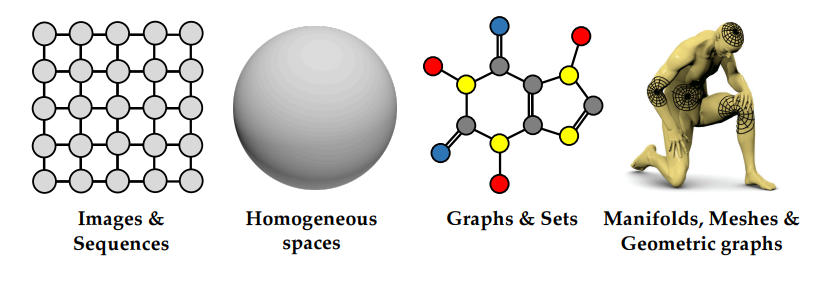
\includegraphics[width=0.7\linewidth]{Images/GDL/gdl_data.png}
    \caption{Ví dụ minh họa về các dạng dữ liệu trong GDL\cite{geometricdeep2022}}
\end{figure}

\vspace{-0.5cm}

Hình \ref{fig:model_gdl} là một số mô hình đã có để xử lý các bài toán khác nhau trong GDL:
\begin{figure}[H]
    \centering
    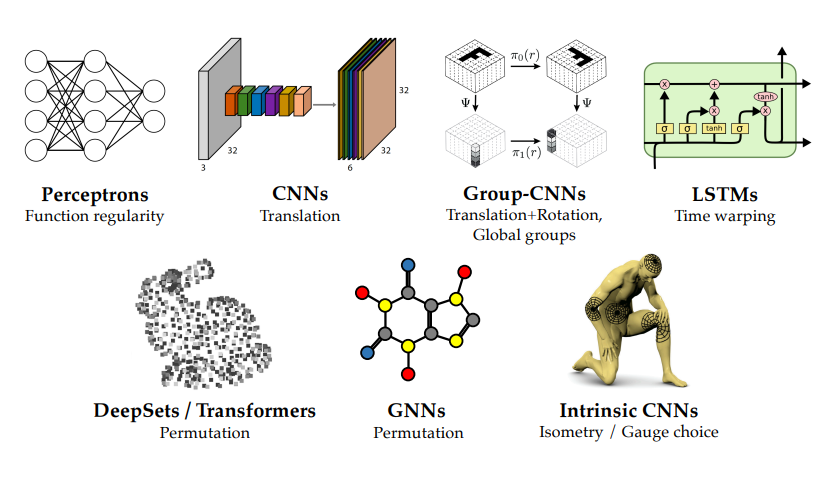
\includegraphics[width=1\linewidth]{Images/GDL/gdl_model_data.png}
    \caption{Các mô hình đã có và tính chất của chúng\cite{geometricdeep2022}}
    \label{fig:model_gdl}
\end{figure}

\subsection{Dữ liệu đồ thị}
Trong thực tế, có rất nhiều bài toán có thể đưa về dạng đồ thị như bài toán liên quan đến phân tử hóa học, mạng xã hội, ... Ta có thể hiểu đồ thị là một hệ thống của các mối liên hệ và sự tương tác - điều này được thể hiện rõ nhất ở cạnh giữa hai đỉnh trong một đồ thị. Để tường minh hơn, Hình \ref{fig:vdgraph} sẽ cho một ví dụ cụ thể hơn:

\begin{figure}[H]
    \centering
    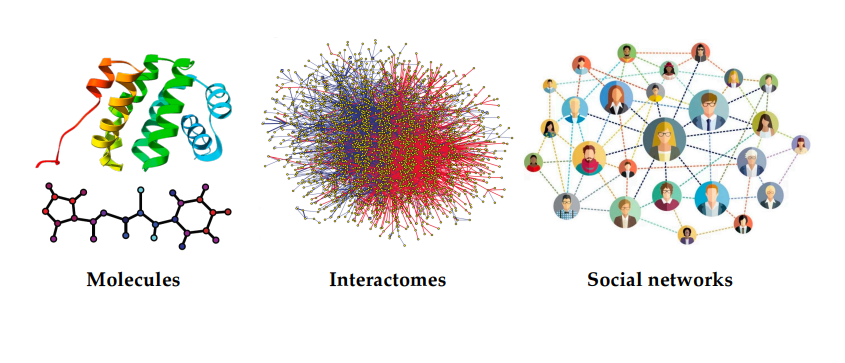
\includegraphics[width=0.7\linewidth]{Images/GDL/graph/graph_vd.png}
    \caption{Ví dụ minh họa về biểu diễn đồ thị của một số dữ liệu thực thế\cite{geometricdeep2022}}
    \label{fig:vdgraph}
\end{figure}

Tuy nhiên, ngoài tập các đỉnh và tập các cạnh của đồ thị ra thì trong mạng nơ-ron đồ thị (GNN) còn thêm một biểu diễn nữa là đặc trưng của các đỉnh. Các đặc trưng này sẽ thể hiện tính chất của các đỉnh ví dụ như đối với mạng xã hội thì là tuổi tác, số lượng bạn bè, ...

\begin{figure}[H]
    \centering
    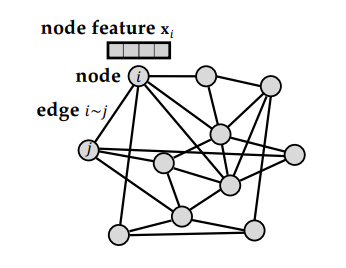
\includegraphics[width=0.7\linewidth]{Images/GDL/graph/graph_represent.png}
    \caption{Minh họa dữ liệu đồ thị trong GNN\cite{geometricdeep2022}}
\end{figure}

Trong GNN, ta có thể đánh số thứ tự các đỉnh tùy ý mà không làm thay đổi cấu trúc của đồ thị, do đó ta cần thiết kết một hàm có đầu vào là đặc trưng các đỉnh và ma trận kề sao cho nó phải bất biến với phép đánh thứ tự các đỉnh. Hay nói cách khác, hàm này phải là một hàm \textit{invariant permutation}. Điều này sẽ giúp cho đặc trưng của các đỉnh sau khi được tổng hợp không bị thay đổi khi ta đánh lại thứ tự các đỉnh.

Tuy nhiên, mặc dù hàm tổng hợp đặc trưng của các đỉnh là bất biến với phép hoán vị nhưng thứ tự các đặc trưng sau khi bị hoán vị vẫn phải thay đổi. Cụ thể hơn, nếu như thứ tự đặc trưng đầu vào bị thay đổi thì thứ tự đặc trưng sau khi tổng hợp đặc trưng cho các đỉnh cũng phải thay đổi, ví dụ: đồ thị có 3 đỉnh thì ta đánh thứ tự là 1, 2, 3 tuy nhiên khi ta hoán vị vị trí các đỉnh là 2, 1, 3 thì sau khi tổng hợp đặc trưng thì thứ tự cũng phải là 2, 1, 3 chứ không phải là 1, 2, 3. Điều này thể hiện tính \textit{equivariant} của GNN.

\begin{figure}[H]
    \centering
    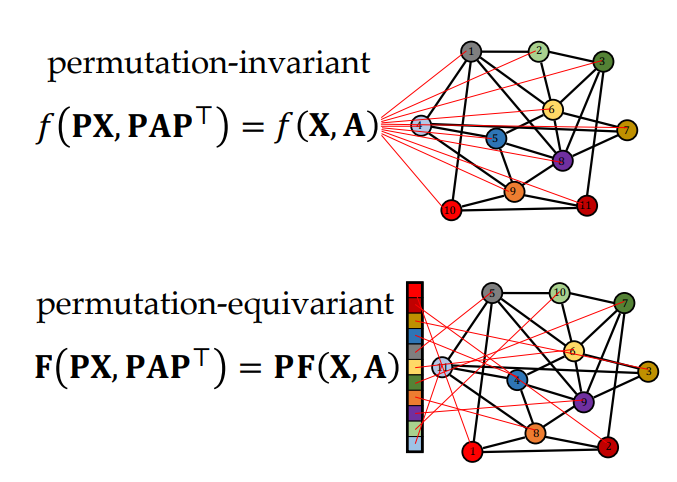
\includegraphics[width=1\linewidth]{Images/GDL/graph/inva_equi_permutation.png}
    \caption{Ảnh minh họa về \textit{invariant} và \textit{equivariant} trong GNN\cite{geometricdeep2022}}
\end{figure}

\begin{figure}[H]
    \centering
    \captionsetup{justification=centering}
    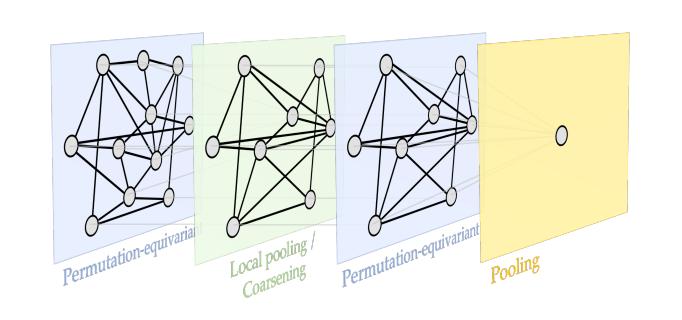
\includegraphics[width=1\linewidth]{Images/GDL/graph/gnn_structure.png}
    \caption{Cấu trúc của một mạng GNN, trong đó pooling là phép ánh xạ đưa một đồ thị thành một vector\cite{geometricdeep2022}}
\end{figure}

\vspace{-0.5cm}

Tiếp theo, báo cáo sẽ đưa ra cấu trúc của một hàm tổng hợp đặc trưng cho một đỉnh trong GNN. Ý tưởng trung của GNN là đặc trưng của một đỉnh sẽ bị ảnh hưởng bởi những đỉnh lân cân và chính nó. Do đó, các cấu trúc GNN khác nhau chỉ là các cách tổng hợp đặc trưng khác nhau và chúng được gọi chung bằng một cái tên là \textit{"message passing"}. 
\begin{figure}[H]
    \centering
    \captionsetup{justification=centering}
    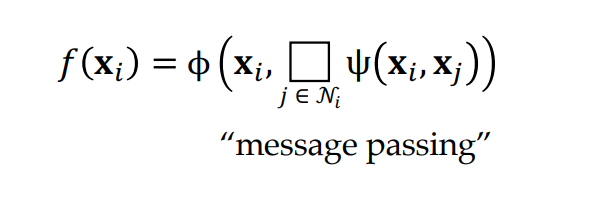
\includegraphics[width=0.7\linewidth]{Images/GDL/graph/message_passing.png}
    \caption{Cấu trúc của \textit{"message passing"} trong GNN, trong đó ô vuông là phép tổng hợp đặc trưng của các lân cận như là phép lấy tổng, trung bình, ...\cite{geometricdeep2022}}
\end{figure}

\vspace{-0.5cm}

Cụ thể hơn, báo cáo sẽ trình bày về hai ví dụ cụ thể của GNN là mạng nơ-ron tích chập (GCN) và mạng nơ-ron chú ý (GAT). Đầu tiên, đối với GCN thì ta chỉ lấy tổng các đặc trưng của lân cận nhân với một trọng số $c_{ij}$ thể hiện mức độ ảnh hưởng đến đỉnh của nó\cite{gcn_paper}. Tuy nhiên hệ số này lại không được tính thông qua bất kì biến nào mà chỉ là một tham số học thông thường. Dó đó, GAT \cite{gat_paper} đã thay thế trọng số $c_{ij}$ thành một hàm tính trọng số với đầu vào là hai đặc trưng của đỉnh hiện tại  $i$ và đỉnh lân cận $j$. Điều này sẽ giúp mô hình có được hệ số chính xác hơn về mức độ ảnh hưởng của các lân cận $j$ đến $i$.

\begin{figure}[H]
    \centering
    \captionsetup{justification=centering}
    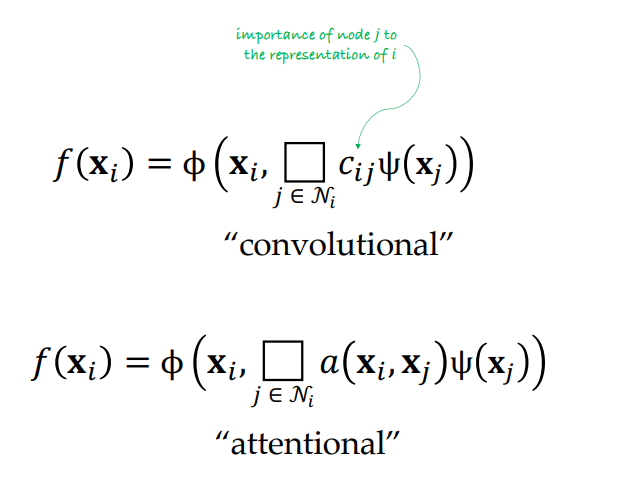
\includegraphics[width=0.7\linewidth]{Images/GDL/graph/gcn_gat.png}
    \caption{Cấu trúc của hàm tổng hợp thông tin của GCN và GAT\cite{geometricdeep2022}}
\end{figure}

Mặc dù GNN thường được biết đến là mạng nơ-ron làm việc với dữ liệu dạng đồ thị nhưng thực tế, nó có một số dạng đặc biệt mà được gọi với tên gọi khác. Dưới đây là một số trường hợp đặc biệt của GNN:

\begin{itemize}
    \item DeepSets\cite{zaheer2018deepsets}: Đây là một mạng nơ-ron làm việc trên tập các điểm ví dụ như point cloud. Do đó, ta có thể coi mạng này là một GNN làm việc với đồ thị không có cạnh.

    \begin{figure}[H]
    \centering
    \captionsetup{justification=centering}
    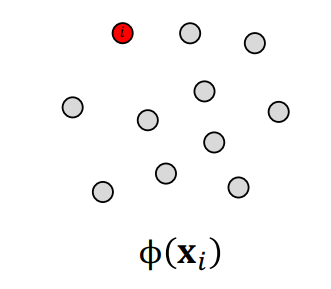
\includegraphics[width=0.4\linewidth]{Images/GDL/graph/deepset.png}
    \caption{Ảnh minh họa DeepSet\cite{geometricdeep2022}}
\end{figure}

    \item Transformers\cite{vaswani2023attentionneed}: Đây là một kiến trúc mạng nơ-ron rất nổi tiếng trong xử lý ngôn ngữ tự nhiên (NLP). Transformers tính hệ số attentions từ một từ đến tất cả các từ khác trong câu. Do đó, nếu ta coi các từ này là một đỉnh của đồ thị và trọng số attention chính là các cạnh thì đây chính là một đồ thị đầy đủ, cho nên, có thể coi Transformers là một mạng GNN làm việc trên đồ thị đầy đủ.

    \begin{figure}[H]
    \centering
    \captionsetup{justification=centering}
    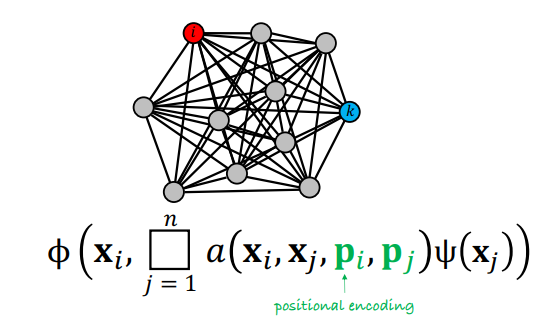
\includegraphics[width=0.7\linewidth]{Images/GDL/graph/transformer.png}
    \caption{Ảnh minh họa Transformer\cite{geometricdeep2022}}
\end{figure}

\end{itemize}

Thông thường đồ thị mà chúng ta làm việc với GNN là chỉ có đặc trưng của các đỉnh mà chưa hề có tọa độ của các đỉnh, ví dụ như đồ thị biểu diễn của một chất hóa học. Do đó, nếu ta làm việc với đồ thị được nhúng vào trong một không gian Euclid, ngoài việc các hàm phải \textit{invariant} và \textit{equivarint} đối với phép hoán vị chỉ số, ta sẽ cần phải thiết kế các hàm \textit{invariant} và \textit{equivarint} đối với các tác động của nhóm phép quay, nghịch đảo, dịch chuyển, phản chiếu\cite{geometricdeep2022}.

\begin{figure}[H]
    \centering
    \captionsetup{justification=centering}
    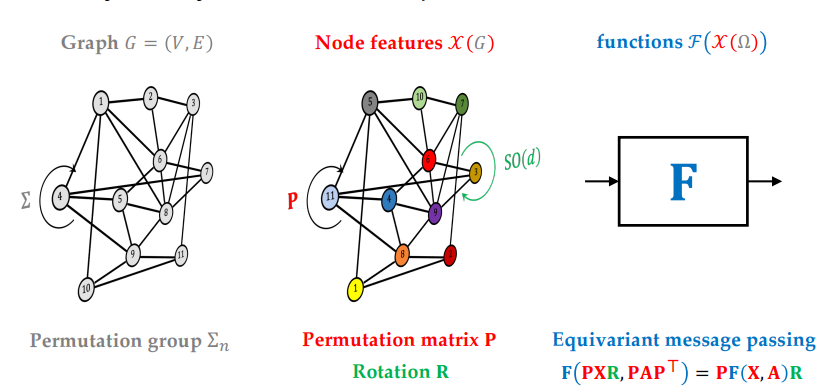
\includegraphics[width=1\linewidth]{Images/GDL/graph/gnn_geometric.png}
    \caption{Ảnh minh họa dữ liệu đồ thị hình học và các phép toán đại số tác động nên nó\cite{geometricdeep2022}}
\end{figure}


\subsection{Dữ liệu đa tạp}
Đa tạp\cite{wikipedia-datap} bản chất là một cấu trúc hình học mà trong đó cục bộ là một không gian Euclid. Ví dụ đơn giản nhất chính là trái đất mà chúng ta đang sống, ta đều biết rằng trái đất có cấu trúc hình học là hình cầu tuy nhiên nếu nhìn cục bộ trên trái đất thì lại là một mặt phẳng (giống như những gì chúng ta nhìn thấy khi đang đứng trên trái đất).

Mặc dù đa tạp có cấu trúc phức tạp nhưng nó lại có tính chất rất quan trong là lân cận. Do đó, để có thể sử dụng các phương pháp học máy để xử lý dạng dữ liệu này thì ta hoàn toàn có thể biểu diễn nó dưới dạng đồ thị, từ đó ta có thể nhúng nó vào một không gian rồi tính toán trên không gian này\cite{geometricdeep2022}. Tuy nhiên đây là cách khá là lâu đời, do đó, ta có thể thực hiện một cách khác là sử dụng GNN lên đồ thị mà không cần phải nhúng đồ thị này vào một không gian nào đó\cite{geometricdeep2022}.

\begin{figure}[H]
    \centering
    \captionsetup{justification=centering}
    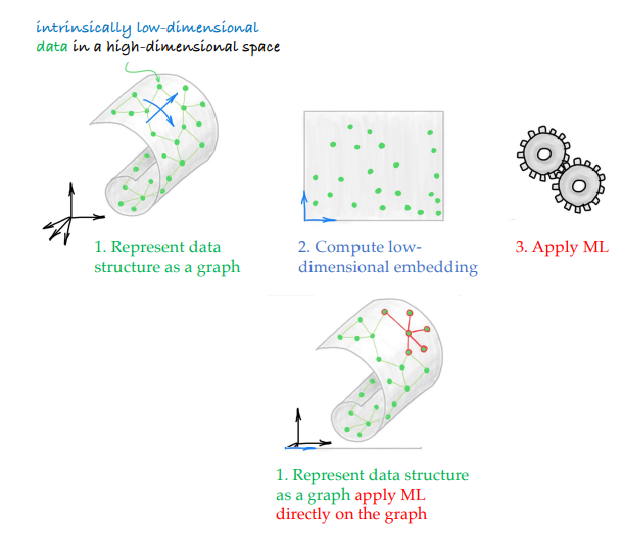
\includegraphics[width=0.7\linewidth]{Images/GDL/graph/manifold.png}
    \caption{Ảnh minh họa hai phương pháp trong \textit{manifold learning}\cite{geometricdeep2022}}
\end{figure}

\subsection{Dữ liệu dạng grid}
Ta có thể coi \textit{grid} là một đồ thị vành (\textit{ring graph})\cite{geometricdeep2022}. Dữ liệu ở dạng này thì các đỉnh sẽ bị cố định cấu trúc lân cận và do đó, ta chỉ cần định nghĩa một hàm tổng hợp đặc trưng cho mỗi đỉnh khá là đơn giản. Hình \ref{fig:grid_ex} là một ví dụ minh họa về \textit{grid}:

\begin{figure}[H]
    \centering
    \captionsetup{justification=centering}
    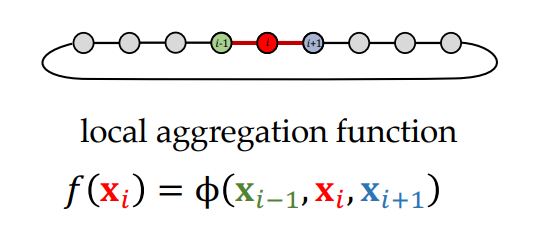
\includegraphics[width=0.7\linewidth]{Images/GDL/graph/grid_ex.png}
    \caption{Ảnh minh họa dữ liệu dạng \textit{grid} và cấu trúc hàm tổng hợp đặc trưng\cite{geometricdeep2022}}
    \label{fig:grid_ex}
\end{figure}

Như ta có thể thấy trong hình \ref{fig:grid_ex} thì hàm tổng hợp đặc trưng chỉ đơn giản là một hàm nhận vào 3 tham số mà không cần đưa input vào một hàm nào khác như GNN. Để tổng quát hơn, ta có thể coi hàm này là tổ hợp tuyến tính của ba tham số đầu vào: $f(x_i) = a x_{i-1} + b x_{i} + c x_{i+1}$ \cite{geometricdeep2022}

\begin{figure}[H]
    \centering
    \captionsetup{justification=centering}
    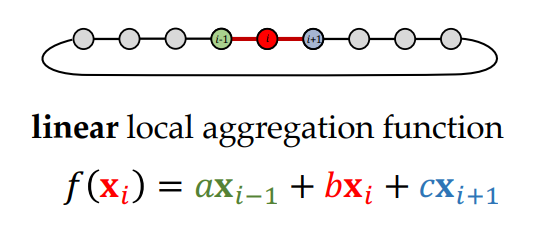
\includegraphics[width=0.7\linewidth]{Images/GDL/graph/grid_agg.png}
    \caption{Ảnh minh họa hàm tổng hợp đặc trưng đối với dữ liệu \textit{grid}\cite{geometricdeep2022}}
\end{figure}





\subsection{Convolution và tính equivarint của nó với phép dịch chuyển}

Để có cái nhìn trực quan và dễ hiểu, báo cáo sẽ lấy ví dụ đối với dữ liệu dạng \textit{grid}. Đối với dạng dữ liệu này, ta có thể tổng quát hóa công thức tổ hợp tuyến tính ở phần trước thành một ma trận \textit{circulant}\cite{geometricdeep2022}. Khi đó, ma trận này chính là một phép tích chập.

\begin{figure}[H]
    \centering
    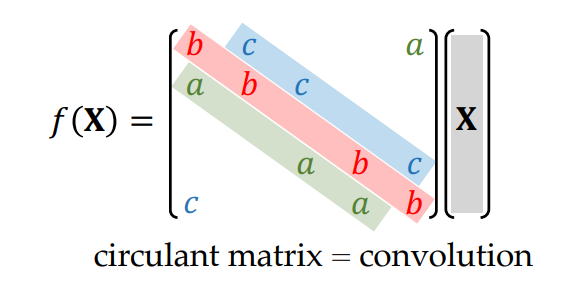
\includegraphics[width=1\linewidth]{Images/GDL/grid_conv/grid_conv.png}
    \caption{Ảnh minh họa về ma trận \textit{circulant}\cite{geometricdeep2022}}
    \label{fig:cir-matrix}
\end{figure}

Hình \ref{fig:cir-matrix} minh họa về phép tính convolution đối với dữ liệu dạng \textit{grid} với những phần để trống là có giá trị bằng 0. Ở đây, ma trận $X$ sẽ là các vector hàng tương ứng với các vector đặc trưng của mỗi đỉnh trong dữ liệu. 

Để chứng minh Convolution equivariant với phép dịch chuyển thì trước hết ta cần xây dựng một ma trận dịch chuyển gọi là \textit{Shift}. Ma trận này sẽ có dạng như hình \ref{fig:shift-matrix}:

\begin{figure}[H]
    \centering
    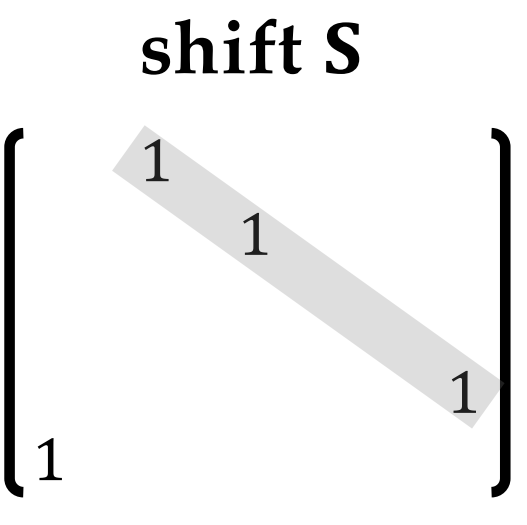
\includegraphics[width=0.4\linewidth]{Images/GDL/grid_conv/shift_matrix.png}
    \caption{Ảnh minh họa về ma trận \textit{Shift}\cite{geometricdeep2022}}
    \label{fig:shift-matrix}
\end{figure}

Ta thấy rằng nếu ta đem ma trận \textit{circulant} (ký hiệu là $C$) nhân với ma trận \textit{Shift} (ký hiệu là S) thì sẽ làm dịch chuyển các giá trị của ma trận \textit{circulant} sang một cột. Tuy nhiên, phép nhân giữa hai ma trận này có một tính chất đặc biệt là giao hoán - nghĩa là $CS = SC$. Tính chất này đã thể hiện tính equivariant của ma trận \textit{circulant} đối với phép dịch chuyển hãy nói rõ hơn thì phép \textit{convolution} equivariant với phép dịch chuyển.

\begin{figure}[H]
    \centering
    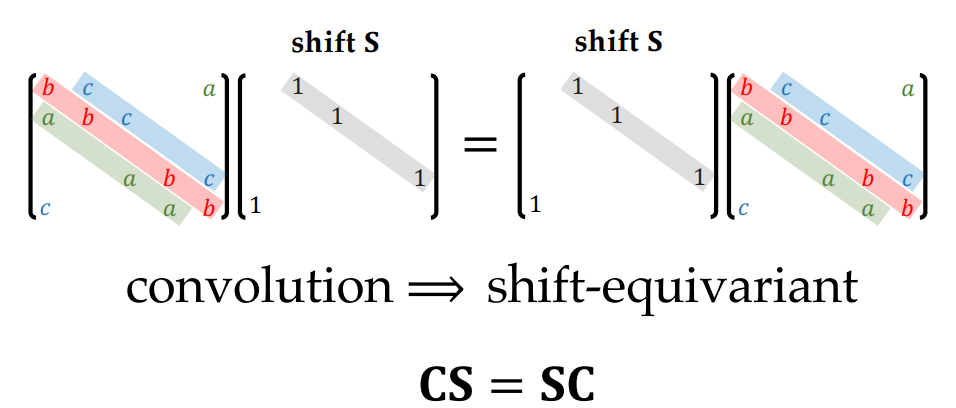
\includegraphics[width=1\linewidth]{Images/GDL/grid_conv/CSSC.png}
    % \caption{Ảnh minh họa về ma trận \textit{Shift}\cite{geometricdeep2022}}
    % \label{fig:shift-matrix}
\end{figure}

Trong đại số tuyến tính có một định lý được phát biểu rằng: "tích của hai ma trận mà có tính giao hoán thì khi ta chéo hóa hai ma trận thì chúng sẽ có chung các vector riêng". Do đó thay vì ta tính vector riêng và giá trị riêng cho ma trận \textit{circulant}, ta hoàn toàn có thể tính chúng thông qua chéo hóa ma trận \textit{Shift} mà ma trận này chéo hóa rất nhanh vì chỉ có giá trị 0 hoặc 1. Điều này giúp ta giảm các phép tính toán đi rất nhiều lần cho việc chéo hóa ma trận \textit{circulant}. Hơn nữa, với mọi ma trận \textit{circulant} khác nhau ta cũng đều có thể dùng chung vector riêng và do đó, ta chỉ cần tính lại giá trị riêng là hoàn thành việc chéo hóa.

\begin{figure}[H]
    \centering
    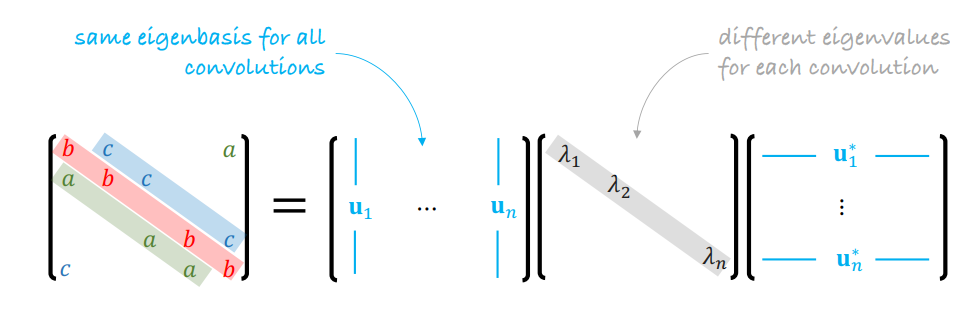
\includegraphics[width=1\linewidth]{Images/GDL/grid_conv/convolution_diagon.png}
    % \caption{Ảnh minh họa về ma trận \textit{Shift}\cite{geometricdeep2022}}
    % \label{fig:shift-matrix}
\end{figure}



\subsection{Mô hình hóa convolution cho không gian tổng quát}
\subsubsection{Tích chập trên miền số thực}

Đầu tiên, báo cáo sẽ mô hình hóa convolution với một ví dụ đơn giải nhất là trên trường số thực. Giả sử ta tính tích chập hai hàm $x$ và $\psi$ kí hiệu là $(x \star \psi)(u)$, khi đó bản chất ta tính tích chập giữa hai hàm này là ta shift hàm $\psi$ trên trục số thực rồi nhân với hàm $x$\cite{geometricdeep2022}, ta kí hiệu phép shift này là $T_u\psi$. Do đó, ta có công thức của phép tính tích chập trên miền số thực như sau:

\begin{center}
    \scalebox{1.5}{($x \star \psi)(u) =  \langle x, T_u \psi \rangle = \int_{-\infty}^{+\infty} x(v)\psi(u-v) dv $}
\end{center}

Để tổng quát hơn, báo cáo sẽ đưa phép shift này thành tác động của nhóm các phép dịch chuyển gọi là $G$, do đó, miền lấy tích phân sẽ là miền giá trị đầu vào của hai hàm $x$ và $\psi$ gọi là $\Omega$. Cuối cùng, ta có công thức sau:

\begin{center}
    \scalebox{1.5}{$(x \star \psi)(g) =  \langle x, \rho(g) \psi \rangle = \int_{\Omega} x(v)\psi(g^{-1}v) dv$}
\end{center}

Tuy nhiên, đây mới chỉ là phép tích chập cho miền số thực, cho nên, tiếp theo báo cáo sẽ trình bày phép tích chập cho các miền không không gian tổng quát hơn.

\subsubsection{Tích chập trên mặt cầu}
Mạng nơ-ron tích chập (CNN) đã trở thành phương pháp được lựa chọn cho các bài toán học liên quan đến ảnh phẳng 2D. Tuy nhiên, một số vấn đề của sự quan tâm gần đây đã tạo ra nhu cầu về các mô hình có thể phân tích hình ảnh hình cầu\cite{cohen2018sphericalcnns}. Ví dụ bao gồm tầm nhìn đa hướng cho máy bay không người lái, robot và ô tô tự hành, bài toán hồi quy phân tử, và mô hình thời tiết và khí hậu toàn cầu. Một ứng dụng đơn giản của mạng tích chập vào phép chiếu phẳng của tín hiệu hình cầu chắc chắn sẽ thất bại, bởi vì các biến dạng thay đổi theo không gian được tạo ra bởi tín hiệu đó một phép chiếu sẽ làm cho việc chia sẻ trọng số tịnh tiến không hiệu quả\cite{cohen2018sphericalcnns}. Do đó, ta sẽ cần phải định nghĩa được phép tích chập mới trên tín hiệu hình cầu.

\begin{figure}[H]
    \centering
    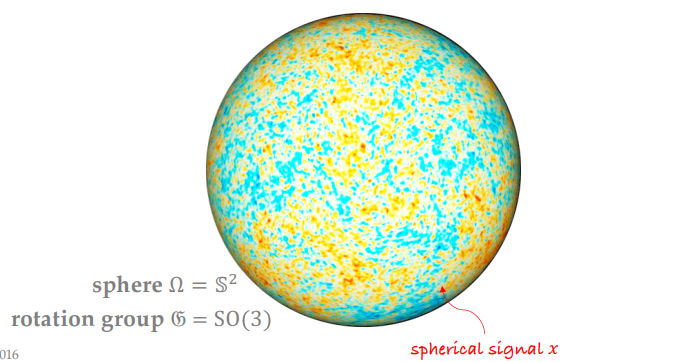
\includegraphics[width=0.7\linewidth]{Images/GDL/sphere_conv/sphere_img.png}
    \caption{Ví dụ minh họa về dữ liệu dạng Sphere\cite{geometricdeep2022}}
\end{figure}

Ta mong muốn có thể định nghĩa tích chập trên miền mặt cầu $S_2$ nhưng khi ta tác động một phép quay lên hình cầu này thì các tín hiệu cầu sẽ bị thay đổi vị trí. Do đó, đầu ra của phép tích chập này sẽ là một hàm theo phép quay $R$:
\begin{center}
    \scalebox{1.5}{$(x\ast \psi )(R)=\int_{S^2}x(u)\psi (R^{-1}u)du$}
\end{center}

Phép quay $R$ ở đây bản chất là ta di chuyển vị trí $u$ đến vị trí $v$ trên mặt cầu $S_2$ và tác động phép quay này chính là tác động của nhóm $SO(3)$. Tuy nhiên, trong $SO(3)$ thì có rất nhiều phép quay để đi từ vị trí $u$ đến vị trí $v$, do đó, ta cần phải tính thêm tích chập trên nhóm $SO(3)$. Khi đó, ta có công thức tính tích chập như sau:

\begin{center}
    \scalebox{1.5}{$((x\ast\psi)\ast\phi)(R)=\int_{SO(3)}(x\ast\psi)(Q)\phi(R^{-1}Q)dQ$}
\end{center}

Để thấy được sự hữu dụng của phép tích chập trên mặt cầu, báo cáo sẽ đưa ra một số ứng dụng củ thể của chúng. Cụ thể hơn, báo cáo sẽ đưa ra một số thực nghiệm của một bài báo nổi tiếng là \textit{Spherical CNN}\cite{cohen2018sphericalcnns}.

Đầu tiên là thực nghiệm so sánh hiệu suất phân loại của \textit{Spherical CNN} với mạng CNN phẳng trên bộ dữ liệu MNIST được chiếu lên mặt cầu. Kết quả cho thấy \textit{Spherical CNN} đạt độ chính xác 96\% trên tập kiểm tra xoay khi được huấn luyện trên tập huấn luyện xoay, trong khi CNN phẳng chỉ đạt 23\%\cite{cohen2018sphericalcnns}. Điều này chứng tỏ khả năng học biểu diễn bất biến xoay vượt trội của \textit{Spherical CNN}.

Tiếp theo, tác giả áp dụng \textit{Spherical CNN} cho bài toán phân loại hình dạng 3D, sử dụng bộ dữ liệu SHREC17 bao gồm các mô hình 3D được xoay ngẫu nhiên. Trên bộ dữ liệu này, \textit{Spherical CNN} đạt điểm F1 là 0.699, chỉ số NDCG là 0.756 và độ chính xác trên tập dữ liệu không xoay là 0.701\cite{cohen2018sphericalcnns}. Kết quả này cho thấy \textit{Spherical CNN} đạt hiệu suất gần như tốt nhất so với các phương pháp hiện đại khác, chứng tỏ tiềm năng của nó trong việc xử lý dữ liệu 3D.

Cuối cùng, tác giả nghiên cứu khả năng của \textit{Spherical CNN} trong việc dự đoán năng lượng nguyên tử hóa của các phân tử dựa trên cấu trúc hình học của chúng. Sử dụng bộ dữ liệu QM7 và biểu diễn các phân tử dưới dạng tín hiệu cầu dựa trên năng lượng Coulomb, \textit{Spherical CNN} đã đạt được RMSE là 8.47 kcal/mol\cite{cohen2018sphericalcnns}. Kết quả này vượt trội hơn hẳn so với các phương pháp dựa trên nhân (RMSE từ 10.82 đến 16.06 kcal/mol) và mạng MLP được huấn luyện trên ma trận Coulomb (RMSE là 12.59 kcal/mol)\cite{cohen2018sphericalcnns}.

\subsubsection{Tích chập cho đa tạp}
Manifold được sử dụng trong nhiều lĩnh vực, đặc biệt là trong học máy và xử lý dữ liệu, vì nó giúp chúng ta hiểu rõ hơn về cấu trúc bên trong của dữ liệu phức tạp. Manifold đặc biệt hữu ích đối với 3D shape (hình dạng 3D) vì nó giúp biểu diễn và xử lý các cấu trúc phức tạp trong không gian 3D một cách hiệu quả hơn. 

Ví dụ, để mô hình một con thỏ theo dạng 3D, ta thường dùng cách khối lập phương chồng lên nhau để mô tả hình dạng và thể tích của chúng (hình ảnh con thỏ bên trái của hình \ref{fig:why-mani}). Tuy nhiên, nếu ta không quan tâm bên trong hình dạng này thì việc biểu diễn bằng các khối lặp phương rất lãng phí không gian lưu trữ và tính toán\cite{geometricdeep2022}. Do đó, đa tạp giúp biểu diễn hình dạng 3D một cách hiệu quả hơn bằng cách tập trung vào các bề mặt của đối tượng, bỏ qua các cấu trúc bên trong không cần thiết.

Do đó, ta có thể sử dụng \textit{manifold} để biểu diễn dữ liệu 3D, nơi chỉ các điểm dữ liệu nằm trên bề mặt của đối tượng 3D được lưu trữ và sử dụng để tạo thành mạng lưới tam giác (mesh). Bởi vậy, \textit{manifold} không "lãng phí" tài nguyên để lưu trữ các cấu trúc bên trong, chỉ tập trung vào bề mặt, từ đó tạo ra một biểu diễn nhẹ và hiệu quả hơn\cite{geometricdeep2022} (hình ảnh con thỏ ở giữa trong hình \ref{fig:why-mani}). Đây cũng là cách được áp dụng trong \textit{computer graphic} liên quan đến vật thể 3D.

Hơn thế nữa, \textit{manifold} được sử dụng như một mô hình tự nhiên cho các hình dạng có thể biến dạng (deformable shapes)\cite{geometricdeep2022}. Ví dụ như hình dạng của con người, với các bộ phận có thể co giãn, di chuyển hoặc thay đổi hình dạng, là một ví dụ điển hình về việc sử dụng manifold (hình ảnh bên phải của hình \ref{fig:why-mani}). Do đó, \textit{manifold} phù hợp với các hình dạng có thể biến dạng, vì nó có thể dễ dàng mô phỏng và điều chỉnh các biến dạng mà không làm mất đi tính toàn vẹn của hình dạng ban đầu\cite{geometricdeep2022}.

\begin{figure}[H]
    \centering
    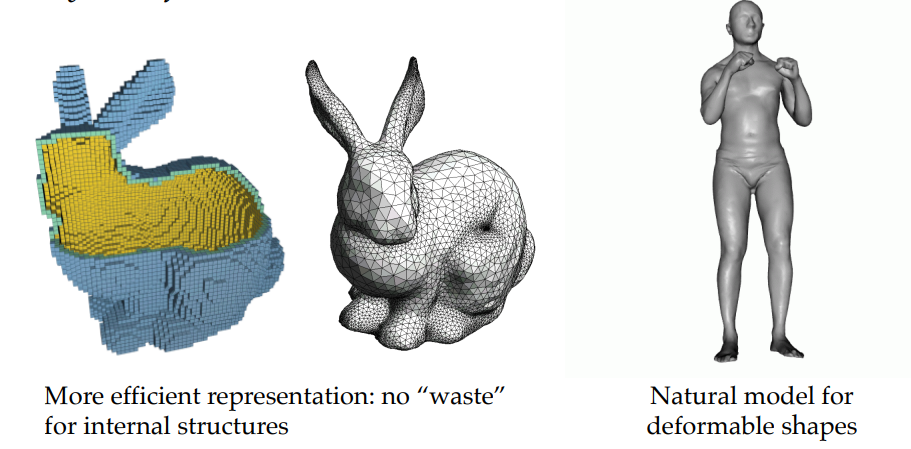
\includegraphics[width=0.8\linewidth]{Images/GDL/manifold_mesh/why_mani.png}
    \caption{Ảnh minh họa dữ liệu đa tạp và meshes\cite{geometricdeep2022}}
    \label{fig:why-mani}
\end{figure}

Tuy nhiên, một ứng dụng quan trọng khác của \textit{manifold} là mô hình hóa protein. Trong quá trình mô hình hóa protein, mục tiêu là biểu diễn các phân tử protein sao cho dễ dàng phân tích các tương tác và biến đổi cấu hình (conformation changes) của chúng. Protein có cấu trúc rất phức tạp với nhiều lớp và các thành phần khác nhau, nhưng không phải tất cả các chi tiết cấu trúc đều quan trọng cho việc nghiên cứu các tương tác chức năng của protein. Dưới đây là hai lý do thể hiện tính hữu ích của \textit{manifold} đối với bài toán này:

\begin{itemize}
    \item Manifold giúp "trừu tượng hóa" (abstract out) các cấu trúc bên trong của protein mà không cần thiết cho việc tương tác. Điều này có nghĩa là chỉ tập trung vào các yếu tố quan trọng như bề mặt của protein, nơi xảy ra các tương tác với các phân tử khác\cite{geometricdeep2022}. Bằng cách này, chúng ta có thể giảm độ phức tạp của mô hình mà không làm mất đi thông tin cần thiết cho việc phân tích.

    \item Protein không phải là những cấu trúc cố định, chúng có thể thay đổi hình dạng hoặc cấu hình để thích ứng với các chức năng sinh học khác nhau. Manifold cung cấp một cách linh hoạt để mô hình hóa những thay đổi này, giữ nguyên tính toàn vẹn của các vùng tương tác quan trọng trong khi cho phép protein thực hiện các biến đổi cấu hình cần thiết\cite{geometricdeep2022}.
\end{itemize}

\begin{figure}[H]
    \centering
    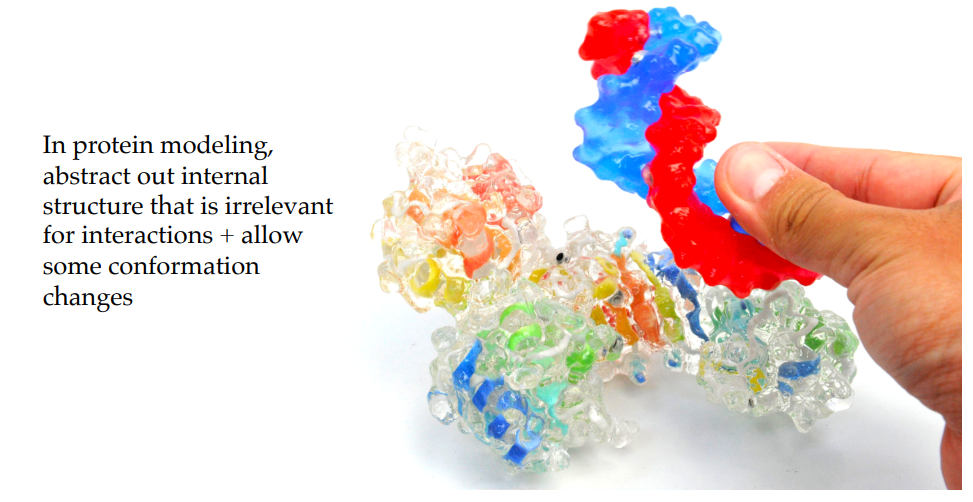
\includegraphics[width=1\linewidth]{Images/GDL/manifold_mesh/protein.png}
    \caption{Ảnh minh họa protein\cite{geometricdeep2022}}
    \label{fig:protein}
\end{figure}

Thông thường, nếu ta sử dụng tích chập trên không gian Euclid thì việc ta di chuyển \textit{filter} từ vị trí A đến vị trí B thì đều sẽ cho kết quả như nhau vì chúng đều đến vị trí B và tính tích chập tại đó (hình \ref{fig:ecnn}). Tuy nhiên, đối với \textit{manifold} thì lại lại khác vì nếu ta đi từ A đến B theo hai con đường khác nhau thì \textit{filter} sẽ bị thay đổi hướng ban đầu và do đó kết quả tính tích chập tại vị trí B sẽ khác nhau. Để thể hiện rõ điều này, báo cáo sẽ đưa ra hai ví dụ sau:
\begin{itemize}
    \item Tích chập trên hình cầu: Hình \ref{fig:sp_cnn_ex} cho thấy hướng của \textit{filter} khác nhau của hai đường đi khác nhau mặc dù chúng có cùng điểm xuất phát và điểm đến.

    \item Tích chập trên mặt \textit{mobius}: Hình \ref{fig:mobius_ex} cho thấy \textit{filter} của đường đi thứ 2 đã bị lật ngược lại so với đường đi đầu tiên mặc dù chúng có cùng điểm xuất phát và điểm đến.
\end{itemize}

\begin{figure}[H]
    \centering
    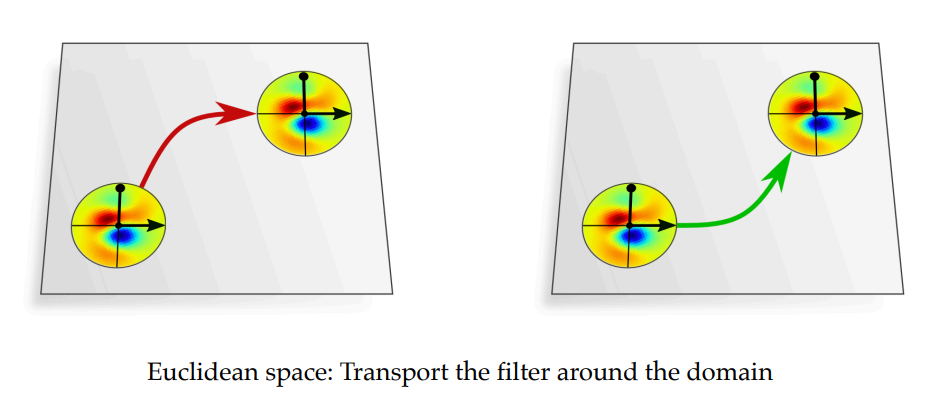
\includegraphics[width=1\linewidth]{Images/GDL/manifold_mesh/E_CNN.png}
    \caption{Ảnh minh họa tích đường đi của \textit{filter} trên không gian Euclid\cite{geometricdeep2022}}
    \label{fig:ecnn}
\end{figure}

\begin{figure}[H]
    \centering
    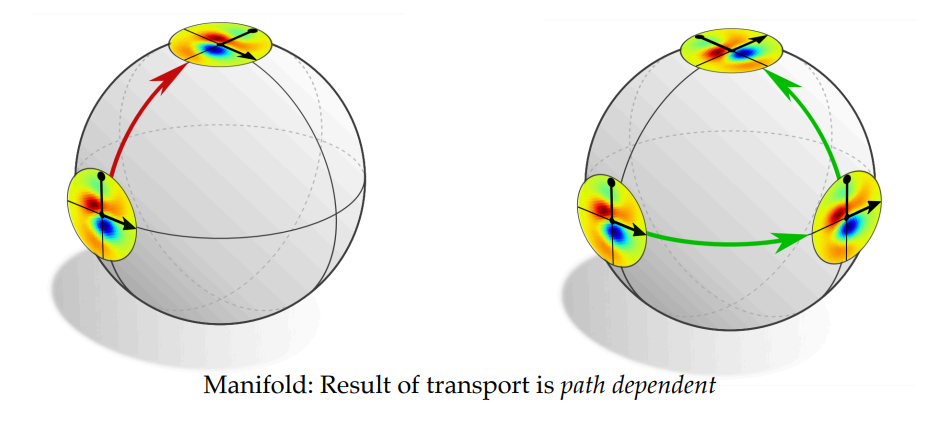
\includegraphics[width=1\linewidth]{Images/GDL/manifold_mesh/sp_cnn_ex.png}
    \caption{Ảnh minh họa tích đường đi của \textit{filter} trên \textit{sphere}\cite{geometricdeep2022}}
    \label{fig:sp_cnn_ex}
\end{figure}

\begin{figure}[H]
    \centering
    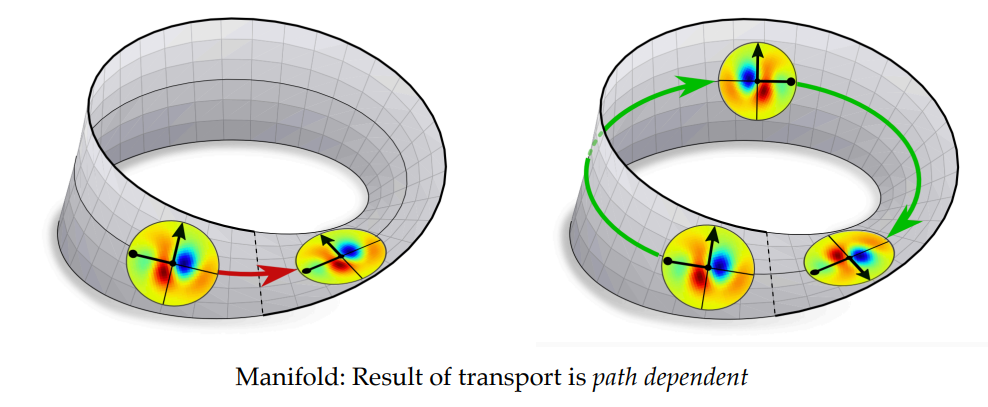
\includegraphics[width=1\linewidth]{Images/GDL/manifold_mesh/mobius_ex.png}
    \caption{Ảnh minh họa tích đường đi của \textit{filter} trên mặt \textit{mobius}\cite{geometricdeep2022}}
    \label{fig:mobius_ex}
\end{figure}

Đối với dữ liệu \textit{manifold}, có hai dạng \textit{invariant} dưới các tác động nhóm như sau:
\begin{itemize}
    \item Biến đổi cục bộ gauge: đây là tác động mà chỉ làm thay đổi tính chất cục bộ của đa tạp mà không ảnh hưởng đến hình dạng tổng thể\cite{geometricdeep2022}. Ví dụ, ta có thể co bóp bụng và điều này làm thay đổi cấu trúc vùng bụng của chúng ta tuy nhiên về mặt tổng thể thì điều này không làm ảnh hưởng đến chúng ta là ai (hình bên trái của hình \ref{fig:local_global_inv}).

    \item Biến đổi toàn cục: đây là tác động làm thay đổi toàn bộ hình dạng của đối tượng, như việc cơ thể người có thể bị kéo giãn, co lại hoặc thay đổi tư thế, tuy nhiên điều này không làm thay đổi đối tượng đấy là gì \cite{geometricdeep2022}. Ví dụ như người A béo lên thì đây chính là tác động làm toàn bộ cơ thể bị thay đổi nhưng về bản chất thì người A vẫn là người A mà không bị biến đổi thành người khác (hai hình bên phải hình \ref{fig:local_global_inv}).
\end{itemize}

\begin{figure}[H]
    \centering
    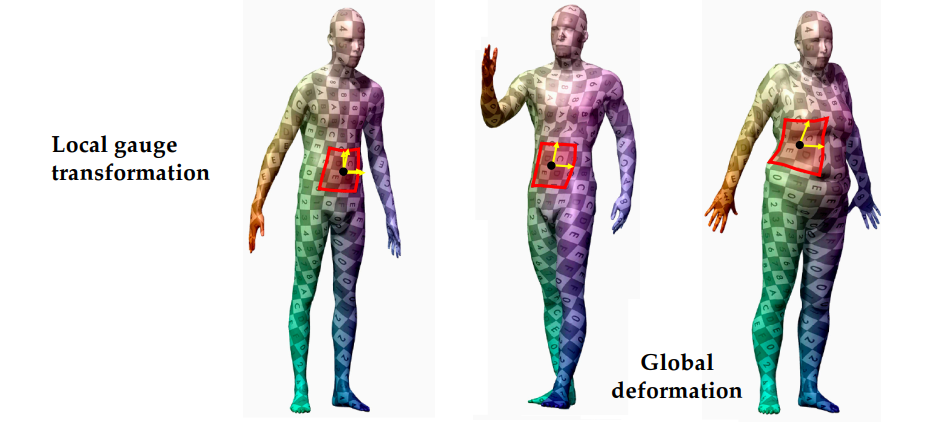
\includegraphics[width=1\linewidth]{Images/GDL/manifold_mesh/local_global_inv.png}
    \caption{Ảnh minh họa hai dạng \textit{invariant} đối với dữ liệu \textit{manifold}\cite{geometricdeep2022}}
    \label{fig:local_global_inv}
\end{figure}

Bây giờ, vấn đề được đặt ra cho việc tính tích chập trên đa tạp là chúng ta cần định nghĩa \textit{filter}. Rất may là đối với đa tạp thì locally ta có thể biểu diễn chúng lên không gian tiếp xúc tại một điểm trên đa tạp (\textit{tangent space}) và nó đẳng cấu với không gian $R^2$. Do đó, ta có thể định nghĩa được filter trên không gian này. Khi đó, ta định nghĩa công thức tính tích chập trên \textit{manifold} như sau:

\begin{center}
    \scalebox{1.5}{$(x \ast \psi)(u) = \int_{T_u \Omega} \psi(v) x(\exp_u v) dv$}
\end{center}
trong đó:
\begin{itemize}
    \item $T_u \Omega$ là không gian tiếp xúc (\textit{tangent space}) tại điểm $u$ trên đa tạp

    \item $\exp_u$ là một phép ánh xạ nội tại nhằm ánh xạ một điểm trong \textit{tangent space} sang một đa tạp $\Omega$
\end{itemize}
tuy nhiên, có một điểm cần lưu ý ở đây là filter của chúng ta sẽ phải invariant với các phép biến đổi đẳng metric (\textit{isometries}).

Ở công thức trên báo cáo đã xây dựng được công thức tính tích chập cho \textit{manifold}, tuy nhiên vector $\mathbf{v}$ trong công thức là một vector trừu tượng, nghĩa là vector này chưa có tọa độ, cho nên phép ánh xạ $\exp_u$ không thể ánh xạ $\mathbf{v}$ sang $manifold$. Do đó, ta cần phải cho $\mathbf{v}$ tọa độ trong $\mathbb{R}^2$ và có một phép biến đổi để ánh xạ $\mathbf{v}$ vào không gian tiếp xúc $T_u \Omega$ - ta gọi phép ánh xạ này là $\omega_u$. Khi đó, ta có công thức tính tích chập sau:
\begin{center}
    \vspace{-0.5cm}
    \scalebox{1.5}{$(x \ast \psi)(u) = \int_{\mathbb{R}^2} \psi(\mathbf{v}) x(\exp_u \omega_u \mathbf{v}) d\mathbf{v}$}
\end{center}
\vspace{-0.5cm}
Tuy nhiên, đây chỉ là công thức cho việc tính tích chập khi chưa có tác động của một nhóm. Do đó, ta sẽ cần xây dựng công thức cho phép biến đổi này, cụ thể hơn là phép biến đổi cục bộ (\textit{gauge transform}). Ta ký hiệu phép biến đổi này như sau:
\begin{center}
    \vspace{-0.5cm}
    \scalebox{1.5}{$g: \Omega \rightarrow SO(2)$}
\end{center}
\vspace{-0.5cm}
Cuối cùng, ta có công thức tính tích chập dưới tác động của một nhóm như sau:
\begin{center}
    \scalebox{1.5}{$(x \star \psi)(u) = \int_{\mathbb{R}^2} \psi(v) \rho(g) x(\exp_u\omega_u v) d{\bf{v}}$}
\end{center}
trong đó, \textit{filter} sẽ phải \textit{equivariant} đối với \textit{gauge transform}, nghĩa là:
\begin{center}
    \scalebox{1.5}{$\psi(g^{-1} {\bf{v}}) = \rho(g^{-1}) \psi({\bf{v}}) \rho(g)$}
\end{center}
\begin{figure}[H]
    \centering
    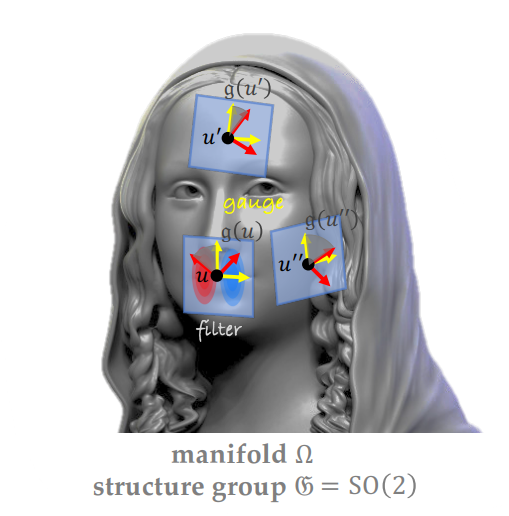
\includegraphics[width=1\linewidth]{Images/GDL/manifold_mesh/mani_cnn/mani_cnn.png}
    \caption{Ảnh minh họa filter trên đa tạp có tác động của một nhóm\cite{geometricdeep2022}}
\end{figure}

Tiếp theo, báo cáo sẽ đưa ra một số ứng dụng thực tế của tích chập trên đa tạp. Một ứng dụng gần gũi với chúng ta nhất đấy là làm đồ họa 3D cho game. Ở đây, việc chúng ta cần làm là chuyển đổi các chuyển động mẫu của khuôn mặt người vào trong đồ họa máy tính.

\begin{figure}[H]
    \centering
    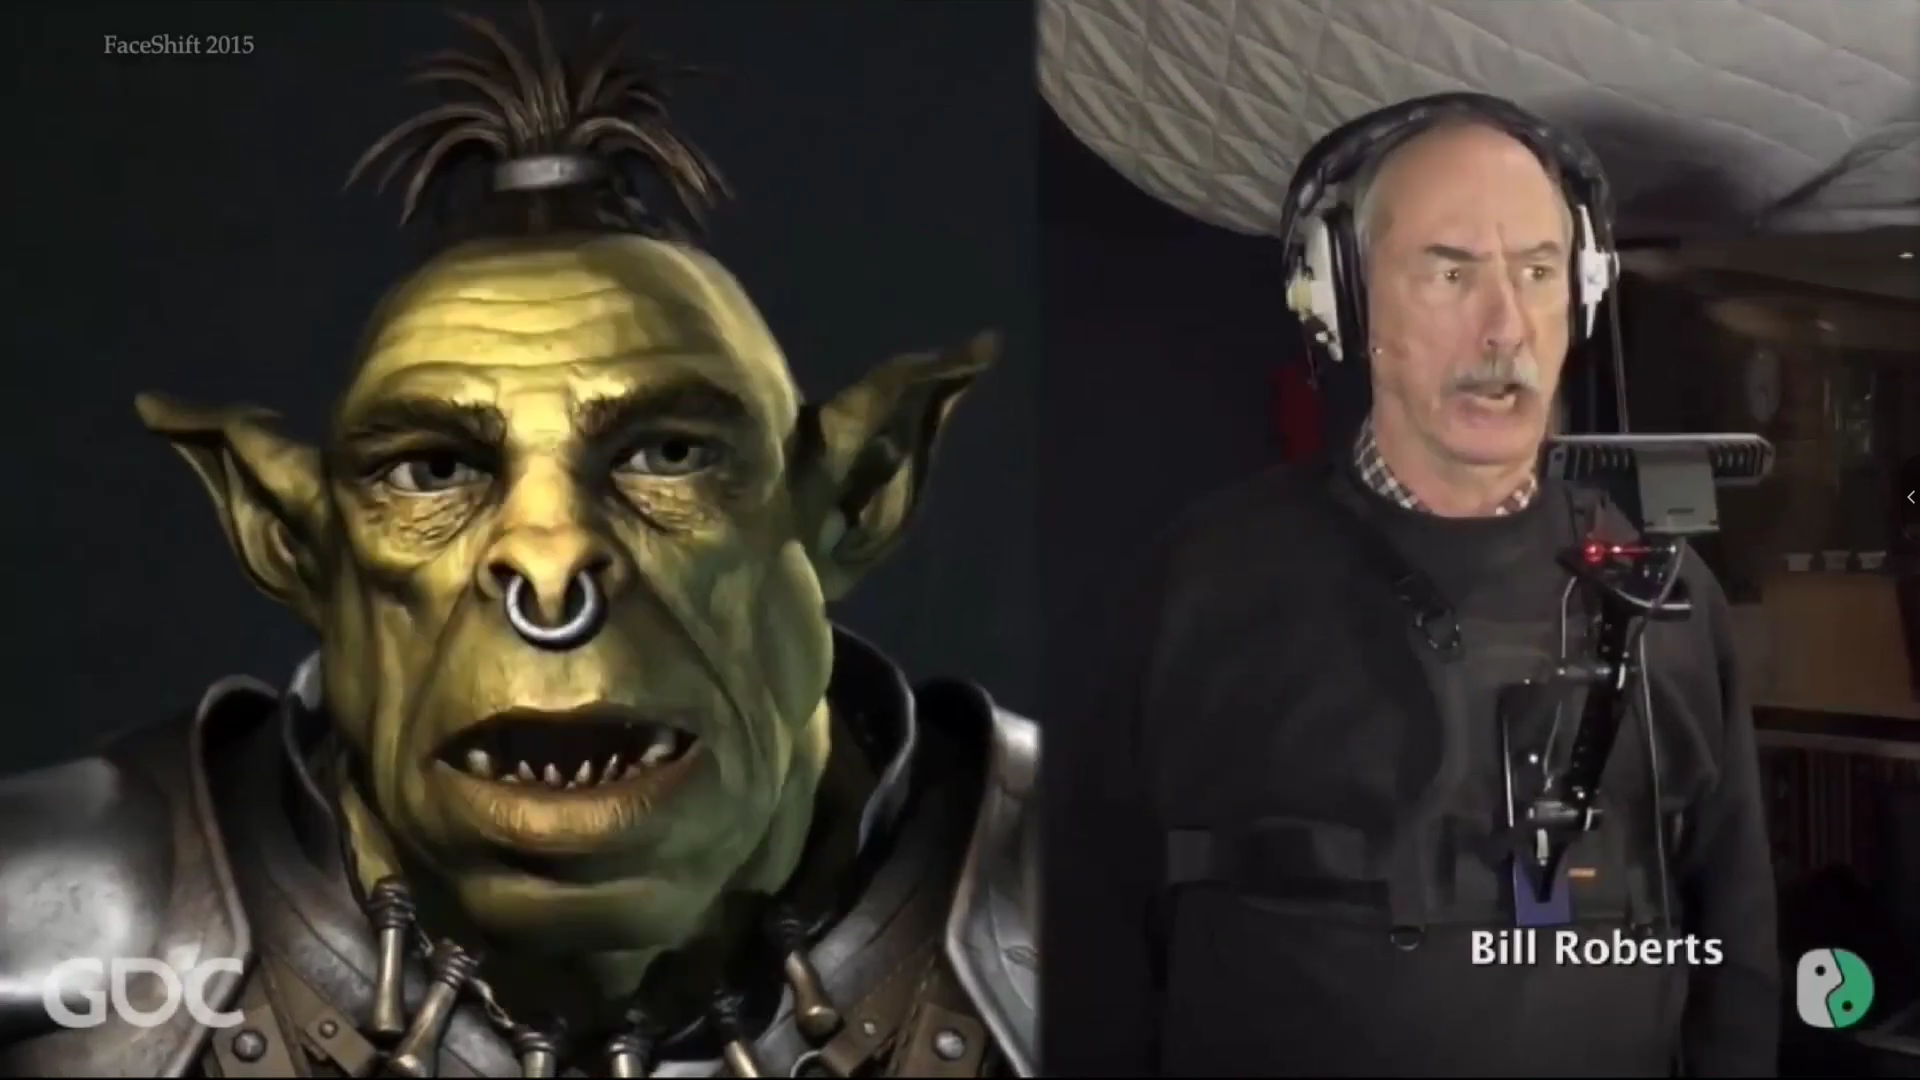
\includegraphics[width=1\linewidth]{Images/GDL/manifold_mesh/mani_cnn/app_mani.png}
    \caption{Ứng dụng của tích chập cho manifold trong computer graphic\cite{geometricdeep2022}}
\end{figure}

Để có thể chuyển được các chuyển động của khuôn mặt sang cho nhân vật trong đồ họa máy tính, đầu tiên là ta sẽ cần phải scan khuôn mặt người thật liên tục để có được input 3D. Khi đó, ta cần ánh xạ đầu vào này vào một khuôn mặt dạng mesh tiêu chuẩn rồi bắt đầu thực hiện các phép biến đổi trên đó để hình thành được chuyển động của khuôn mặt. Tuy nhiên, đầu vào 3D sau khi scan có khá là nhiều nhiễu và do đó, ta cần phải sử dụng mesh-convolution để có thể ánh xạ chính xác nhất có thể từ đầu vào sang khuôn mặt dạng mesh tiêu chuẩn\cite{geometricdeep2022}.

\begin{figure}[H]
    \centering
    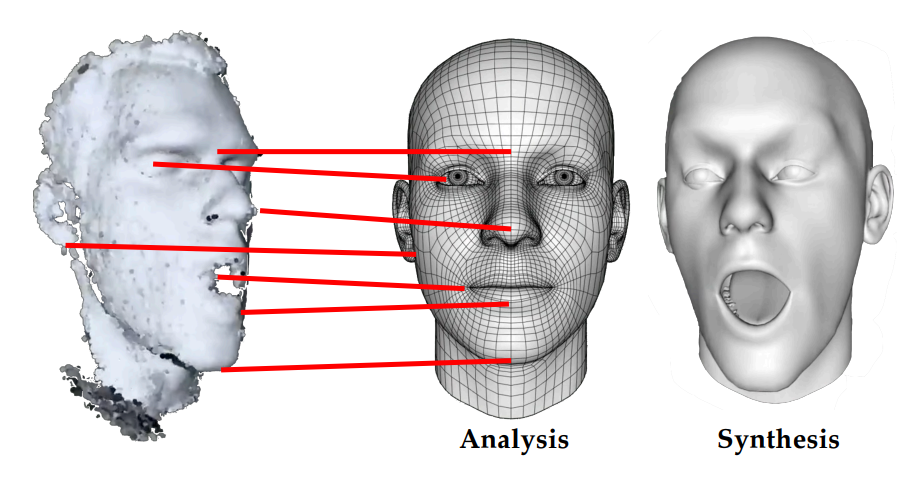
\includegraphics[width=1\linewidth]{Images/GDL/manifold_mesh/mani_cnn/computer_graphic.png}
    \caption{Tổng quan quá trình đưa chuyển động của khuôn mặt vào trong đồ họa máy tính\cite{geometricdeep2022}}
\end{figure}

Một ứng dụng khác của tích chập trên đa tạp đó là tái cấu trúc lại hình dạng 3D từ một hình ảnh 2D. Nghĩa là đầu vào sẽ là một hình ảnh và đầu ra sẽ là hình dạng 3D của vật thể trong hình ảnh đấy\cite{geometricdeep2022}.

\begin{figure}[H]
    \centering
    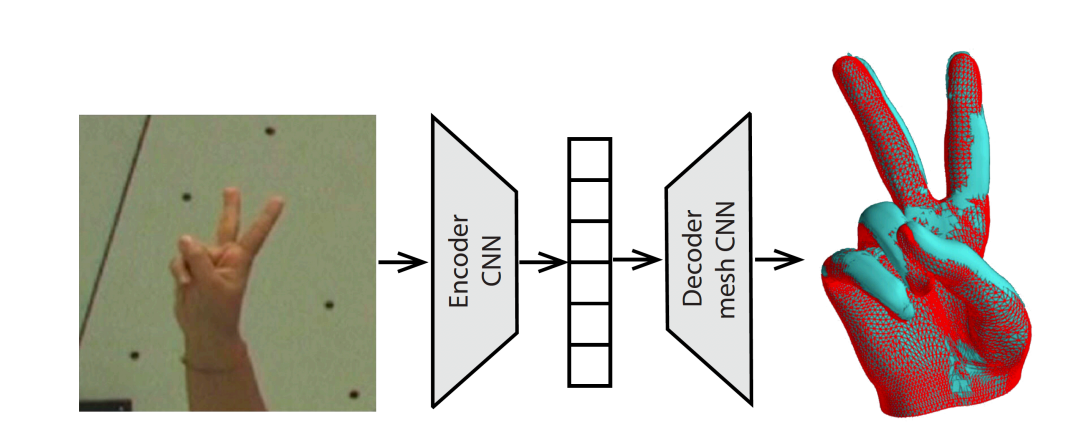
\includegraphics[width=1\linewidth]{Images/GDL/manifold_mesh/mani_cnn/3d_hand.png}
    \caption{Ứng dụng tái cấu trúc lại hình dạng 3D của một vật thể từ một hình ảnh\cite{geometricdeep2022}}
\end{figure}


\section{Geometric Deep learning cho AMR trong NLP}
\textbf{Lưu ý:} đây chỉ là lý thuyết báo cáo tự đề xuất ra cho nên vẫn chưa được kiểm chứng hoàn toàn.

Abstract Meaning Representation (AMR) là một dạng biểu diễn ngữ nghĩa trừu tượng, dùng để mô tả ý nghĩa của câu theo cách ngôn ngữ độc lập\cite{amr-guidelines}. AMR tập trung vào việc biểu diễn cấu trúc ngữ nghĩa của câu dưới dạng đồ thị, trong đó các đỉnh là các khái niệm hoặc thực thể, và các cạnh biểu diễn mối quan hệ giữa các khái niệm này.

AMR nắm bắt được “ai đang làm gì với ai” trong một câu. Mỗi câu được biểu diễn dưới dạng một đồ thị có gốc, có hướng, và không chu trình với các nhãn trên các cạnh (quan hệ) và các lá (khái niệm)\cite{amr-guidelines}.

Giống như một cây phân tích cú pháp, AMR cung cấp một cấu trúc duy nhất có thể duyệt qua mà tính đến tất cả các từ. Nó không phải là một tập hợp các lớp chú thích rời rạc. Không giống như cây phân tích cú pháp, AMR là trừu tượng. Nó có thể biểu diễn nhiều câu ngôn ngữ tự nhiên khác nhau. AMR không chú thích các từ riêng lẻ trong một câu, như một phân tích phụ thuộc\cite{amr-guidelines}.

\begin{figure}[H]
    \centering
    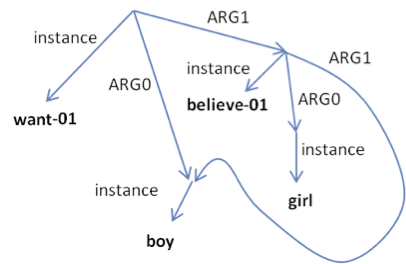
\includegraphics[width=1\linewidth]{Images/GDL/amr_ex.png}
    \caption{Ví dụ minh họa về AMR\cite{amr-guidelines}}
    \label{fig:ex_amr}
\end{figure}

Câu AMR trong hình \ref{fig:ex_amr} có nghĩa là: Có một sự kiện mong muốn, trong đó ARG0 (người mong muốn) là một cậu bé, và ARG1 (điều được mong muốn) là một sự kiện tin tưởng. Sự kiện tin tưởng này có ARG0 (người tin tưởng), là một cô gái, và nó có ARG1 (điều được tin tưởng), chính là cậu bé vừa được nhắc đến. Ở đây, cậu bé đóng hai vai trò: (1) là ARG0 của "want-01", và (2) là ARG1 của "believe-01". AMR thể hiện điều này bằng hai cạnh có hướng trỏ đến cùng một nút. (Theo OntoNotes, các giác quan của vị ngữ được đánh dấu bằng hậu tố như -01 và -02, trong khi ARG0, ARG1, v.v., chỉ các vai trò cốt lõi, cụ thể của vị ngữ.)

\begin{figure}[H]
    \centering
    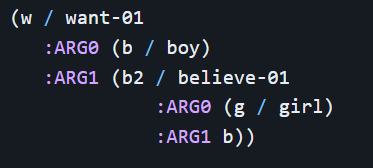
\includegraphics[width=1\linewidth]{Images/GDL/amr_ex_text.png}
    \caption{Biểu diễn AMR dạng text của ví dụ trong hình \ref{fig:ex_amr}}
\end{figure}

Kể từ khi ra đời, AMR đã được áp dụng rộng rãi trong nhiều lĩnh vực xử lý ngôn ngữ tự nhiên. Các ứng dụng phổ biến bao gồm dịch máy, tóm tắt văn bản, trả lời câu hỏi, và phân tích cảm xúc. Sự đa dạng trong ứng dụng này chứng tỏ tính linh hoạt và hữu ích của AMR trong việc nắm bắt và biểu diễn ý nghĩa ngôn ngữ.

Song song với sự phát triển về ứng dụng, nhiều công cụ đã được tạo ra để hỗ trợ việc tự động hóa quá trình tạo và phân tích AMR. Các công cụ này bao gồm các bộ phân tích cú pháp tiên tiến và các mô hình học máy phức tạp, giúp tăng cường khả năng xử lý AMR ở quy mô lớn.

Mặc dù ban đầu AMR được phát triển chủ yếu cho tiếng Anh, nhưng theo thời gian, nó đã được mở rộng để hỗ trợ nhiều ngôn ngữ khác. Điều này đã mở ra cơ hội cho việc áp dụng AMR trong các nhiệm vụ xử lý ngôn ngữ đa ngôn ngữ và liên ngôn ngữ.

Quá trình phát triển của AMR vẫn đang tiếp diễn. Các nhà nghiên cứu liên tục cải tiến và mở rộng khả năng của AMR để xử lý các hiện tượng ngôn ngữ ngày càng phức tạp hơn, đồng thời tăng độ chính xác trong biểu diễn ngữ nghĩa. Những nỗ lực này nhằm đảm bảo rằng AMR vẫn là một công cụ mạnh mẽ và linh hoạt trong lĩnh vực xử lý ngôn ngữ tự nhiên, có khả năng đáp ứng các thách thức mới nổi trong việc hiểu và biểu diễn ngôn ngữ tự nhiên.

Trong lĩnh vực dịch máy, AMR đóng vai trò quan trọng như một biểu diễn trung gian. Bằng cách chuyển đổi văn bản nguồn thành AMR, sau đó từ AMR sang ngôn ngữ đích, các hệ thống dịch có thể nắm bắt được ý nghĩa sâu sắc của văn bản, giúp tạo ra bản dịch chính xác và tự nhiên hơn. Phương pháp này đặc biệt hiệu quả khi xử lý các cặp ngôn ngữ có cấu trúc khác biệt lớn.

AMR cũng được sử dụng rộng rãi trong tác vụ tóm tắt văn bản. Bằng cách biểu diễn nội dung chính của văn bản dưới dạng đồ thị AMR, các hệ thống có thể dễ dàng xác định và trích xuất thông tin quan trọng, từ đó tạo ra các bản tóm tắt ngắn gọn và đầy đủ nội dung.

Trong lĩnh vực trả lời câu hỏi, AMR giúp phân tích cả câu hỏi và các đoạn văn bản tiềm năng chứa câu trả lời. Việc so sánh cấu trúc AMR của câu hỏi và văn bản cho phép hệ thống xác định chính xác thông tin cần thiết để đưa ra câu trả lời phù hợp.

AMR cũng được ứng dụng trong phân tích cảm xúc và khai thác ý kiến. Bằng cách biểu diễn cấu trúc ngữ nghĩa của câu, AMR giúp hệ thống nắm bắt được các sắc thái tinh tế trong cảm xúc và quan điểm được thể hiện, vượt ra ngoài phân tích đơn thuần dựa trên từ khóa.

Trong lĩnh vực sinh văn bản tự động, AMR được sử dụng như một khuôn mẫu ngữ nghĩa. Các hệ thống có thể tạo ra văn bản mạch lạc và có ý nghĩa bằng cách sinh câu từ biểu diễn AMR, đảm bảo rằng nội dung được tạo ra phù hợp với ý định ngữ nghĩa mong muốn.

Ngoài ra, AMR còn được áp dụng trong nhiều lĩnh vực khác như phân tích diễn ngôn, trích xuất quan hệ, và hệ thống đối thoại. Trong mỗi trường hợp, khả năng nắm bắt ý nghĩa sâu sắc của AMR giúp cải thiện hiệu suất và độ chính xác của các hệ thống xử lý ngôn ngữ tự nhiên.

Tiếp theo, báo cáo sẽ đưa ra hai ví dụ về AMR của hai câu đồng nghĩa sau:

- "The scientist who discovered the new element won the Nobel Prize and inspired young researchers around the world."

- "The Nobel Prize was awarded to the scientist who found the new element, and this achievement motivated young researchers globally."

\begin{figure}[H]
    \centering
    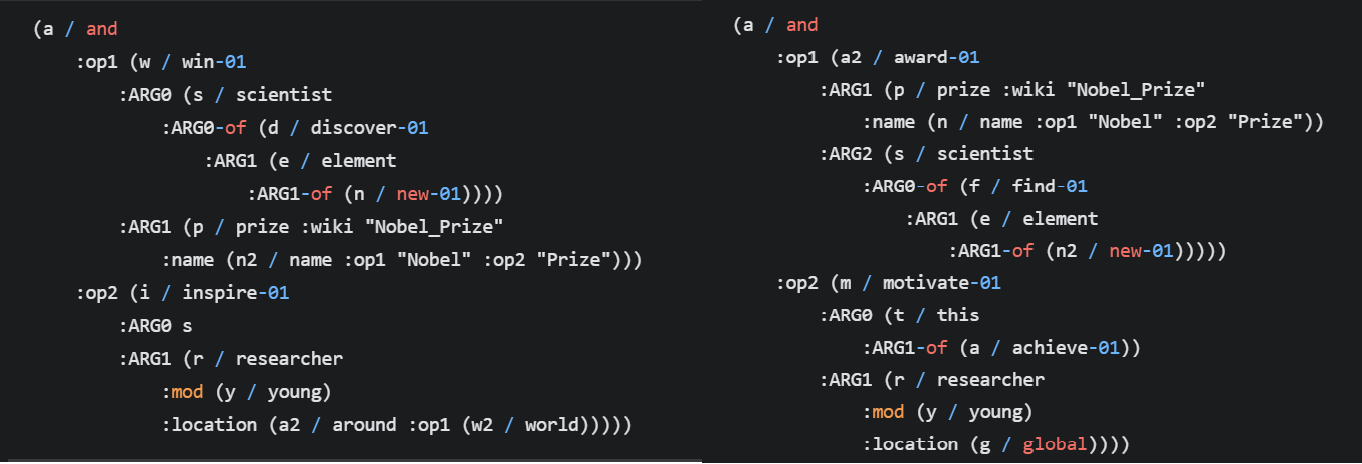
\includegraphics[width=1\linewidth]{Images/GDL/amr_2_sym.png}
    \caption{Biểu diễn AMR của hai câu đồng nghĩa}
    \label{fig:amr_sym}
\end{figure}

Từ hình \ref{fig:amr_sym} có thể thấy rằng cả hai AMR đều thể hiện được hai sự kiện chính: việc một nhà khoa học được trao giải Nobel vì phát hiện ra nguyên tố mới, và việc thành tựu này truyền cảm hứng/thúc đẩy các nhà khoa học trẻ. Bên cạnh đó, các thực thể chính (nhà khoa học, giải Nobel, nguyên tố mới) đều được xác định rõ ràng trong cả hai AMR. Mối quan hệ ngữ nghĩa giữa các thực thể cũng được thể hiện rõ ràng bằng các nhãn vai trò ngữ nghĩa (ARG0, ARG1, ARG0-of, ARG1-of, mod, location).

Tuy nhiên, hai AMR có sự khác biệt về cấu trúc. AMR bên trái sử dụng cấu trúc phức tạp hơn với nhiều mệnh đề con lồng nhau, trong khi AMR bên phải có cấu trúc đơn giản hơn với hai mệnh đề chính được nối với nhau bởi "and".

Sự lựa chọn động từ trung tâm để diễn tả sự kiện được trao giải Nobel cũng khác nhau. AMR bên trái sử dụng động từ "win" (chiến thắng), trong khi AMR bên phải sử dụng "award" (trao thưởng). Việc lựa chọn động từ này ảnh hưởng đến cấu trúc và cách thức thể hiện vai trò ngữ nghĩa trong mỗi AMR.

Phạm vi ảnh hưởng của sự kiện "truyền cảm hứng/thúc đẩy" cũng được thể hiện khác nhau. Trong khi AMR bên trái thể hiện sự kiện "truyền cảm hứng" có phạm vi ảnh hưởng là "các nhà khoa học trẻ trên toàn thế giới", thì AMR bên phải lại thể hiện sự kiện "thúc đẩy" có phạm vi ảnh hưởng là "toàn cầu" (không chỉ giới hạn ở các nhà khoa học trẻ).

Cuối cùng, vị trí của thông tin về phạm vi ảnh hưởng cũng khác nhau. AMR bên trái đặt thông tin về phạm vi ảnh hưởng ("around the world") ở cuối câu, trong khi AMR bên phải đặt thông tin này ("globally") gần với động từ "motivate".

Như vậy, có thể thấy rằng với hai câu khác nhau nhưng cùng ý nghĩa thì khi ta chuyển sang AMR thì sẽ cho ta hai đồ thị AMR khác nhau. Hệ quả, nên tồn tại một quan hệ xác suất giữa hai đồ thị AMR trong một văn cảnh nào đấy. 

Do đó, không gian các đồ thị AMR có thể đưa ra ý tưởng về một cấu trúc mới. Hãy xem xét khái niệm tương đương (equivalence) như một tập hợp các mũi tên: có thể đảo ngược và có thể kết hợp (composable). Điều này dẫn đến việc hình thành một cấu trúc groupoid (groupoid structure). Tuy nhiên, ngoài cấu trúc groupoid, còn có nhiều cấu trúc khác có thể áp dụng. Ví dụ, ta có thể định nghĩa một hàm trên đồ thị AMR để mô tả tần suất sử dụng các phần tử trong đồ thị.

\begin{figure}[H]
    \centering
    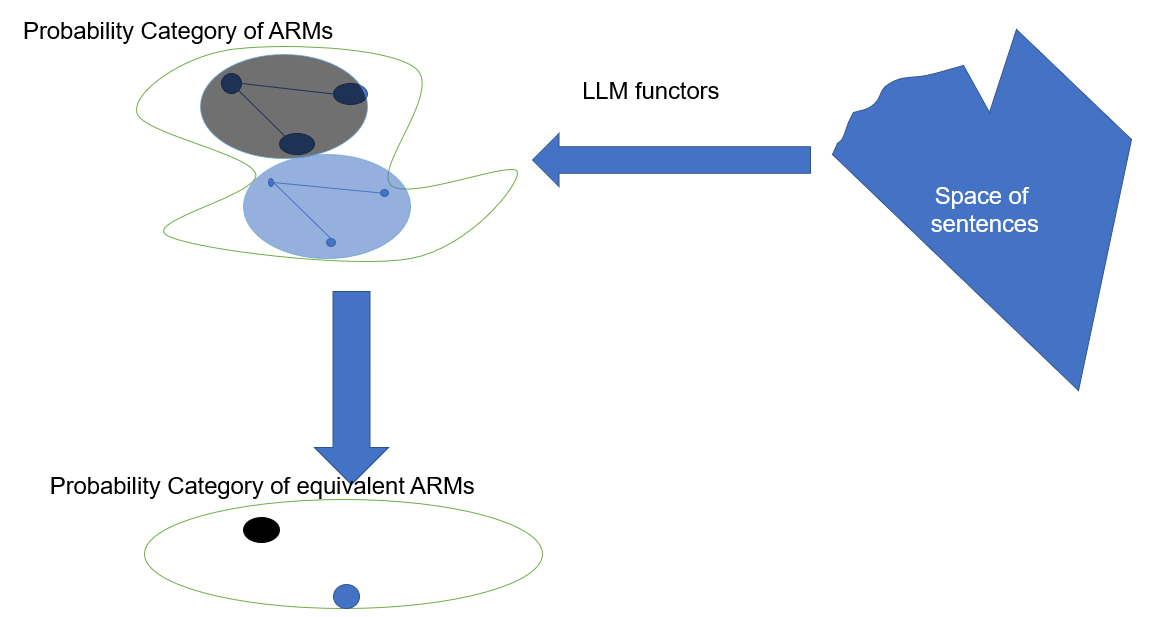
\includegraphics[width=1\linewidth]{Images/GDL/new_AMR_structure.png}
    \caption{Ý tưởng cấu trúc mới về AMR. (LLM functors nghĩa là sử dụng LLM để chuyển một câu sang AMR)}
\end{figure}

Ngoài ra, việc so sánh các đồ thị AMR từ các câu đồng nghĩa cũng mở ra hướng nghiên cứu về các phép biến đổi giữa các đồ thị này. Chúng ta có thể xem xét cách các đồ thị AMR biến đổi khi có sự thay đổi trong cách diễn đạt ngôn ngữ tự nhiên, từ đó xây dựng các mô hình dự đoán hoặc phân loại dựa trên các biến đổi này. Điều này không chỉ giúp hiểu rõ hơn về cấu trúc ngữ nghĩa mà còn có thể ứng dụng trong việc cải thiện các mô hình ngôn ngữ, như mô hình dịch máy hoặc tóm tắt văn bản, bằng cách khai thác sự tương quan giữa các biểu diễn AMR khác nhau trong ngữ cảnh cụ thể.

Sự kết hợp (compose) của các hàm tử (functors) tạo ra các dạng tương đương AMR mới chưa được ghi nhận trong tài liệu hiện có, và những tương đương này có thể được tính toán một cách tự động thông qua mô hình ngôn ngữ lớn (Large Language Model).

Tiếp theo, báo cáo sẽ lấy một ví dụ dịch một câu sang các ngôn ngữ khác nhau rồi dịch trở lại ngon ngữ ban đầu (hình \ref{fig:amr_trans}).

\begin{figure}[H]
    \centering
    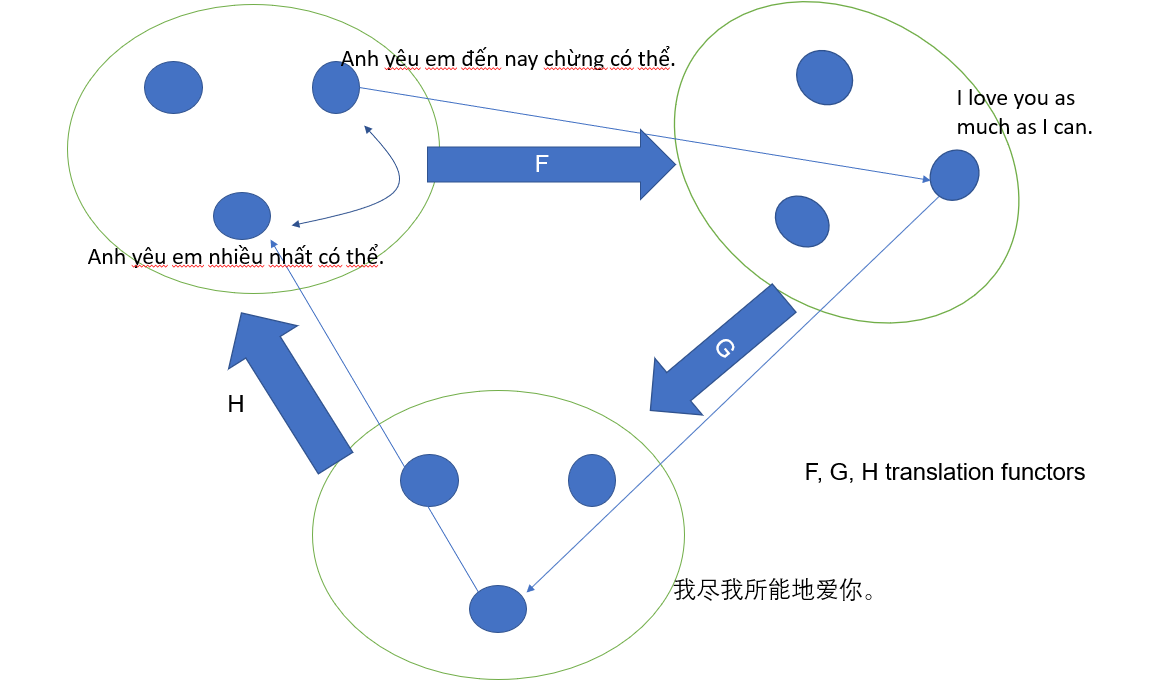
\includegraphics[width=1\linewidth]{Images/GDL/amr_translation.png}
    \caption{Ví dụ minh họa bằng dịch một câu sang ngôn ngữ khác. Những điểm trong hình tròn là các câu khác nhau nhưng cùng nghĩa. F, G, F là các phép dịch một ngôn ngữ này sang ngôn ngữ khác.}
    \label{fig:amr_trans}
\end{figure}
Từ hình \ref{fig:amr_trans} cho thấy trong quá trình dịch và biểu diễn ngữ nghĩa của câu qua nhiều ngôn ngữ. Khi một câu được dịch qua các ngôn ngữ khác nhau (được biểu thị bằng các hàm ánh xạ F, G, H) rồi quay trở lại ngôn ngữ ban đầu, kết quả thu được thường là một câu mới nhưng vẫn giữ nguyên ý nghĩa cốt lõi của câu gốc.

Các hàm ánh xạ F, G, H được coi là các phép biến đổi 1-1 giữa các không gian ngôn ngữ. Tuy nhiên, khi xét đến không gian biểu diễn ngữ nghĩa trừu tượng như AMR (Abstract Meaning Representation), phép nâng (lifting) không còn là phép đồng nhất (identity) mà chỉ còn là phép tương đương (equivalence).

Điều này có nghĩa là các đồ thị AMR của các câu đồng nghĩa, dù có thể khác nhau về cấu trúc cụ thể, nhưng vẫn nên có một mức độ tương đồng nhất định. Ta có thể quantify mức độ tương đồng này bằng một xác suất hay độ đo tương đương nào đó.

Hiện tượng này phản ánh bản chất phức tạp của ngôn ngữ tự nhiên, nơi cùng một ý nghĩa có thể được diễn đạt bằng nhiều cách khác nhau, không chỉ trong cùng một ngôn ngữ mà còn qua các ngôn ngữ khác nhau. Nó cũng cho thấy sự cần thiết của các phương pháp biểu diễn ngữ nghĩa linh hoạt như AMR, có khả năng nắm bắt được bản chất ngữ nghĩa của câu mà không bị ràng buộc quá chặt vào cấu trúc cú pháp cụ thể.

Cuối cùng, nhận xét này gợi ý rằng trong các ứng dụng xử lý ngôn ngữ tự nhiên, đặc biệt là trong lĩnh vực dịch máy và so sánh ngữ nghĩa giữa các câu, ta nên tập trung vào việc phát triển các phương pháp đánh giá độ tương đồng ngữ nghĩa dựa trên các biểu diễn trừu tượng như AMR, thay vì chỉ dựa vào sự giống nhau về mặt từ vựng hay cú pháp.

\begin{figure}[H]
    \centering
    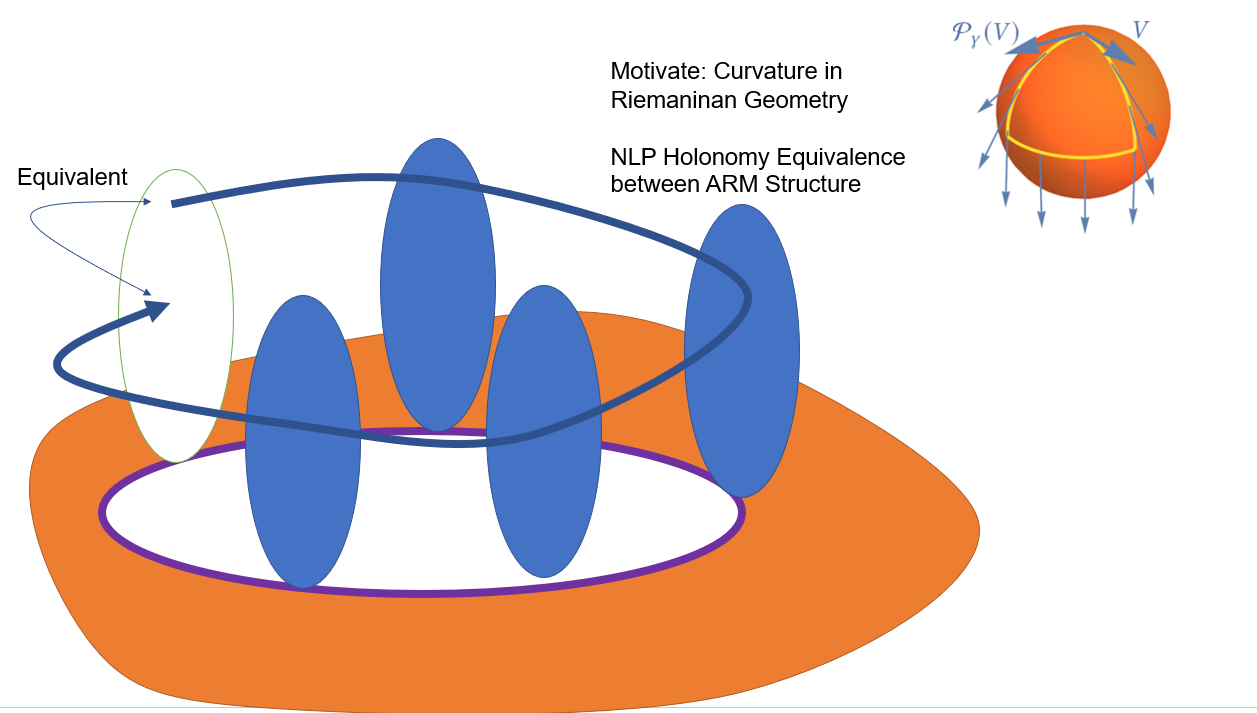
\includegraphics[width=1\linewidth]{Images/GDL/Riemanian_motivation.png}
    \caption{Motivation từ Curvature in Riemaninan Geometry cho cấu trúc AMR trong NLP}
\end{figure}

% \section{Phân loại hình 3D sử dụng TFN}
% \subsection{Tổng quan bài toán}
Bài toán của báo cáo là phân loại hình 3D. Cụ thể hơn thì báo cáo sẽ làm việc về bài toán Point Cloud classification. Point Cloud Classification là một bài toán trong lĩnh vực Machine Learning và Computer Vision, đặc biệt liên quan đến việc xử lý dữ liệu 3D. Point Cloud là một tập hợp các điểm trong không gian ba chiều (3D), mỗi điểm được xác định bởi tọa độ (x, y, z) và đôi khi kèm theo các thông tin khác như màu sắc, cường độ ánh sáng, hay các đặc điểm khác. Các điểm này được thu thập từ các cảm biến 3D như LiDAR, máy quét 3D, hoặc từ các hình ảnh 2D thông qua các kỹ thuật như Structure from Motion (SfM).

Mục tiêu của bài toán Point Cloud Classification là phân loại toàn bộ đám mây điểm thành các nhãn (labels) khác nhau, chẳng hạn như xác định một đám mây điểm thuộc về một loại đối tượng nào đó (ví dụ: ô tô, người, cây cối, tòa nhà).

\begin{figure}[H]
    \centering
    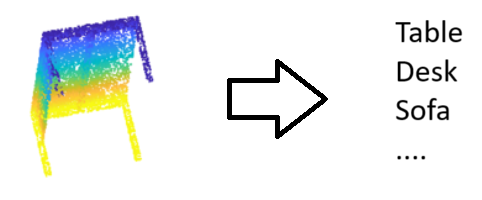
\includegraphics[width=0.7\linewidth]{Images/tong_quan_bt.png}
\end{figure}

Một số thách thức chính trong Point Cloud Classification bao gồm:
\begin{itemize}
    \item Không gian đầu vào có kích thước lớn: Đám mây điểm thường chứa hàng nghìn đến hàng triệu điểm, gây khó khăn cho việc xử lý và tính toán.

    \item Thiếu thông tin cấu trúc: Khác với hình ảnh 2D có cấu trúc lưới cố định, các điểm trong point cloud không có thứ tự cố định và không có cấu trúc mạng lưới rõ ràng, làm cho việc áp dụng các phương pháp truyền thống như Convolutional Neural Networks (CNN) trở nên khó khăn.

    \item Tính không đồng nhất: Point cloud có thể có mật độ không đồng nhất, nghĩa là một số vùng có thể chứa nhiều điểm hơn các vùng khác, tạo ra sự bất đối xứng trong dữ liệu.

\end{itemize}

\subsection{Dữ liệu sử dụng}
Ở đây, báo cáo sẽ sử dụng bộ dữ liệu về Point Cloud là bộ dữ liệu ModelNet10\cite{data_modelnet10}. ModelNet10 là một bộ dữ liệu chuẩn trong lĩnh vực xử lý dữ liệu 3D, được sử dụng phổ biến trong các nghiên cứu và thí nghiệm liên quan đến Point Cloud Classification và 3D Object Recognition. Bộ dữ liệu này được giới thiệu lần đầu tiên bởi các nhà nghiên cứu tại Princeton University trong bài báo "3D ShapeNets: A Deep Representation for Volumetric Shapes"\cite{data_modelnet10} vào năm 2015.

\begin{figure}[H]
    \centering
    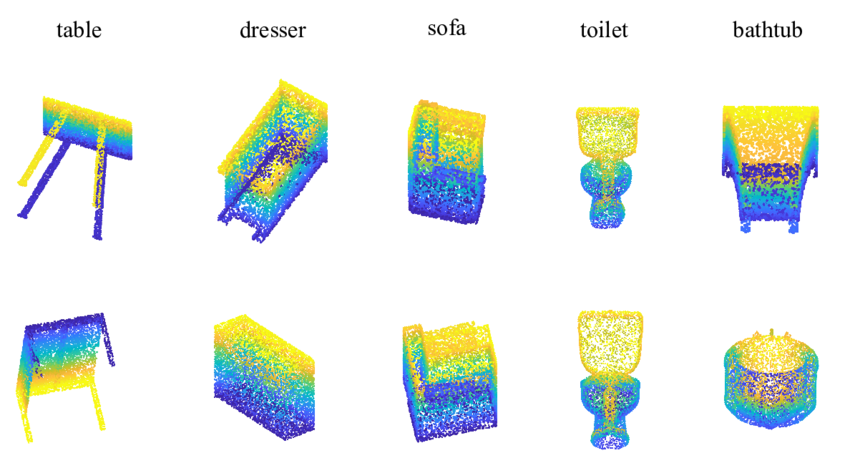
\includegraphics[width=0.8\linewidth]{Images/TFN/data_img.png}
    \caption{Ảnh minh họa một số dữ liệu trong tập dữ liệu ModelNet10}
\end{figure}

ModelNet10 bao gồm khoảng \textbf{3991} dữ liệu 3D được trích xuất từ các đối tượng trong thế giới thực và được sắp xếp thành 10 danh mục khác nhau. Những danh mục này bao gồm: Bed (Giường), Chair (Ghế), Desk (Bàn làm việc), Dresser (Tủ ngăn kéo), Monitor (Màn hình), Nightstand (Tủ đầu giường), Sofa (Ghế sofa), Table (Bàn), Toilet (Bồn cầu), Bathtub (Bồn tắm)

\subsection{Phương pháp thực nghiệm}
Ở đây, báo cáo sẽ chỉ thực nghiệm để thấy được sự hữu ích của các mạng \textit{equivariant deep learning} trong bài toán liên quan đến dữ liệu 3D. Cụ thể hơn, báo cáo chỉ sử dụng TFN để cho thấy rằng dữ liệu được training là dữ liệu chưa xoay đi một góc nào đấy. Do đó, sau khi training xong, báo cáo sẽ xay dữ liệu một cách ngẫu nhiên rồi sau đó cho mô hình dự đoán.

Về phần dữ liệu, do hạn chế về mặt phần cứng là 15GB VRAM của Google Colab, báo cáo không thể training hết được toàn bộ dữ liệu do có một số dữ liệu có rất nhiều điểm (khoảng hơn 1000 điểm). Do đó, với mỗi loại nhãn của dữ liệu, báo cáo sẽ lấy một điểm dữ liệu cho mỗi loại nhãn rồi sau đó training mô hình TFN với dữ liệu này.

Về phần mô hình, báo cáo sử dụng thư viện E3NN để xây dựng mô hình TFN. TFN sẽ có hai layer do số lượng dữ liệu ít (10 dữ liệu). Giữa hai layer này sẽ có một hàm kích hoạt của thư viện E3NN có tên là Gate. Kích thước đầu ra cuối cùng sẽ là 10 với hàm kích hoạt là Softmax tượng trưng cho xác suất mà một dữ liệu thuộc vào từng class. 

Mô hình sẽ được huấn luyện với 200 epochs với kích thước batch là 10. Hàm mất mát được sử dụng là Cross-Entropy loss và thuật toán tối ưu là Adam với learning rate là $10^{-3}$.

\begin{table}[h!]
\centering
 \begin{tabular}{|c | c |} 
 \hline
    Thiết bị huấn luyện & T4 GPU (Google Colab)\\
 \hline
    Số epochs & 200\\
 \hline
    Kích thước batch & 10\\
 \hline
    Hàm mất mát & Cross - Entropy\\
 \hline
    Thuật toán tối ưu & Adam\\
 \hline
    Hệ số học & $10^{-3}$\\
 \hline
 \end{tabular}
 \caption{Bảng thống kê các thông số huấn luyện mô hình}
\end{table}

\subsection{Kết quả thực nghiệm và đánh giá}
Sau quá trình training, mô hình đạt được độ chính xác là 80\% . Điều này cho thấy rằng mô hình vẫn chưa phân loại tốt hoàn toàn vì một phần là thiếu dữ liệu hoặc có thể là do có một số dữ liệu có cấu trúc khá là tương đồng nên mô hình chưa thể nhận biết được. Hình \ref{fig:acc_track} dưới đây là biểu đồ theo dõi chất lượng dự đoán của mô hình.

\begin{figure}[H]
    \centering
    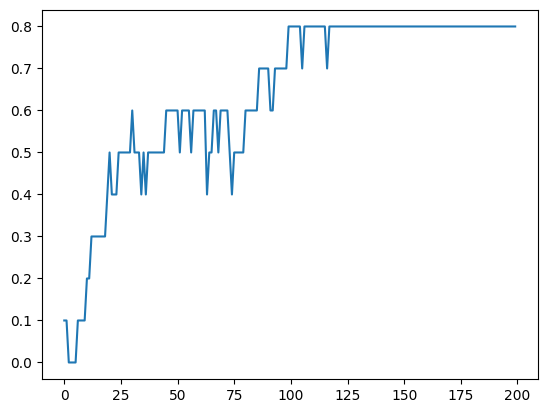
\includegraphics[width=0.7\linewidth]{Images/TFN/acc_re.png}
    \caption{Biểu đồ theo dõi tính độ chính xác của mô hình trong quá trình training}
    \label{fig:acc_track}
\end{figure}

Từ biểu đồ có thể thấy độ chính xác ban đầu khá thấp nhưng tăng dần qua các epoch, cho thấy mô hình đang học và cải thiện dần. Tuy nhiên, trong quá trình training, độ chính xác dao động khá nhiều, đặc biệt là ở giai đoạn giữa, điều này có thể chỉ ra rằng mô hình phải tinh chỉnh khá nhiều để khớp với dữ liệu hơn. Cuối quá trình training, độ chính xác dần ổn định và đạt mức khoảng 0.8, nghĩa là mô hình có khả năng dự đoán đúng khoảng 80\% dữ liệu.

Để thấy được độ hiệu quả của mô hình khi dự đoán dữ liệu đối với tác động của phép xoay, báo cáo sẽ xoay từng dữ liệu một góc bất kỳ trong không gian 3 chiều rồi cho mô hình dự đoán. Hình \ref{fig:equi_re} cho thấy cái nhìn tổng quan về hiệu suất của mô hình với các hình có tiêu đề chỉ có chữ label là dữ liệu gốc còn đối với dữ liệu còn lại là dữ liệu đã được xoay.

\begin{figure}[H]
    \centering
    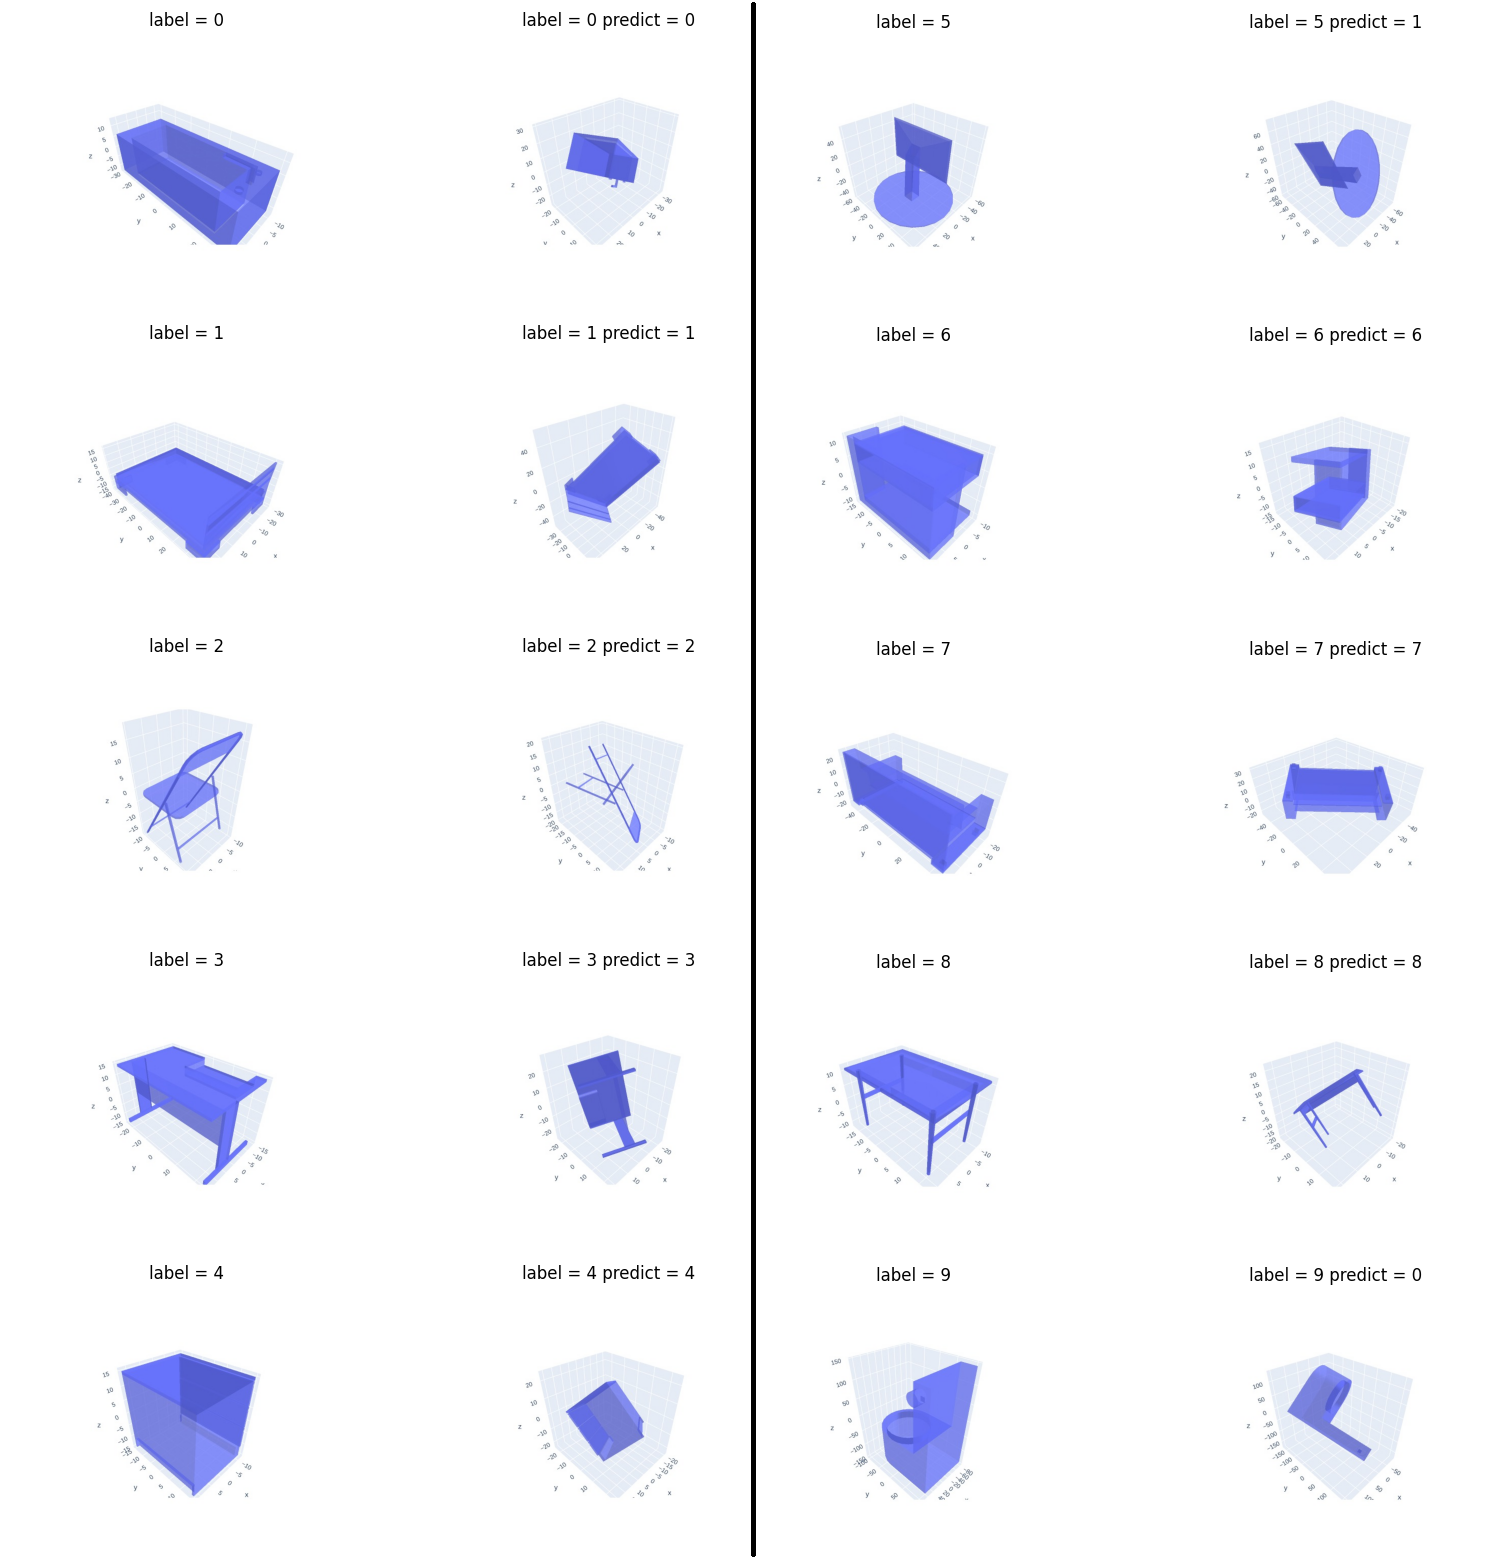
\includegraphics[width=1\linewidth]{Images/TFN/result.png}
    \caption{Hình ảnh thống kê kết quả dự đoán của mô hình}
    \label{fig:equi_re}
\end{figure}

Có thể thấy mô hình hoạt động khá tốt khi dự đoán chính xác 8/10 dữ liệu. Đối với những dữ liệu dự đoán sai thì chúng ta sẽ cần phải thêm dữ liệu đối với mô hình hoặc là thay đổi cấu trúc của mô hình để đạt được hiệu quả cao hơn.